\section{Mono-jet model implementation}


There are several matrix element implementations of the
DM production through spin-0 and spin-1 mediators.

For a spin-1 mediator, the implementation in \powheg generates
DM pair production with 1 parton at next-to-leading order (NLO), whilst \madgraph and \mcfm are at leading order (LO)~\footnote{Spin-0 and spin-1 mediator models will also be provided 
in the near future to the same precision in \madgraph~\cite{Alwall:1405.0301}.}. As shown in \powheg Ref.\,\cite{Haisch:2013ata}, including NLO corrections result in an enhancement in the cross section as compared to LO and though this is not significant, it does lead to a substantial reduction in the dependence on the choice of the renormalization and factorization scale and hence the theoretical uncertainty on the signal prediction. 
Since NLO calculations are available for the process in \powheg, we recommend to proceed with \powheg as the generator of choice. 

For a spin-0 mediator, the top-quark loop is the most important
consideration.
The matrix element implementation of the \schannel spin-0 mediated DM production is available in \mcfm~\cite{Fox:2012ru,Harris:2014hga} and \powheg~\cite{Haisch:2015ioa} with the full top-loop calculation at LO.
The \powheg and \mcfm implementations include the finite
top quark mass dependence for DM pair production with 1 parton at LO.
For consistency with the spin-1 generation, we recommend using \powheg
for this case as well.

Here, we document some specific settings needed to run the \powheg 
generation for the Dark Matter models.

\begin{itemize}
\item \powheg can handle the generation of events (be it at LO or NLO) 
in two different modes explained in the following. The second one 
is the recommended one. The relevant keywords in the input card are 
\bornsuppfact and \bornktmin. 

\begin{enumerate}
\item unweighted events: %keywords

\bornsuppfact: negative or absent\\
\bornktmin <PT>

This runs the program in the most straightforward way,
but most likely it is not the more convenient choice, as will be
explained below. \powheg will generate unweighted events using a sharp
lower cut (with value \texttt{PT}) on the leading-jet \pT. Since this is a
generation cut, the user should make sure that the value used for
\bornktmin is lower than the actual analysis cut to be eventually
used. It is good practice to use as a value in the input card a
transverse momentum 10-20\% smaller than the final analysis cut, and
check that the final result is independent, by exploring an even
smaller value of \bornktmin. The drawback of this running mode is that
it's difficult to populate well and in a single run both the low-\pT
region as well as the high-pt tail.

\item weighted events: %keywords

\bornsuppfact <PTS>\\
\bornktmin <PT>

\powheg will now produce weighted events, thereby allowing to generate
a single sample that provides sufficient statistics in all signal
regions. Events are still generated with a sharp lower cut set by
\bornktmin, but the \bornsuppfact parameter is used to set the event
suppression factor according to

\begin{equation}
F(\kT)=\frac{\kT^2}{\kT^2+\bornsuppfact^2} \;.
\end{equation}

In this way, the events at, for instance, low \MET, are suppressed
but receive an higher weight, which ensures at the same time higher
statistics at high \MET. We recommend to set \bornsuppfact to 1000.

The \bornktmin parameter allows to suppress the low \MET region
even further by starting the generation at a certain value of \kT also
in this runnning mode. It is recommended to set this parameter to half
the lower analysis \MET cut. For instance for the event selection used in the
CMS/ATLAS monojet analyses, assuming the lowest \MET region being defined above 300\,GeV, the proposed value for
\bornktmin is 150.  However, this parameter should be set keeping in
mind the event selection of all the analyses that will use these
signal samples and hence a threshold lower than 150 may be required.

\end{enumerate}

\Todo{Emanuele:``On the usage of fixed or running width. It is my opinion that one
should use fixed widths. Although clearly there are limitations, I
think this goes into the direction of making all as simple and
transparent as possible. Moreover, all the discussions in the last
months aw well as the large majority of runs were done with fixed
widths. Since there was some interest over the last couple of weeks,
here is my suggestion for the powheg section.''}

%\begin{itemize}
\item Remove the \runningwidth keyword, or set it to 0, which is the
  default value. Running with fixed widths is the recommended
  option. Although there are limitations, this is the more
  straightforward, simple and transparent option, and it was used for
  Forum studies. 

  While not recommended, the alternative, a running width for the
  propagator of the s-channel mediator, can be selected by setting
  runningwidth to 1. In this case the denominator of the mediator's
  propagator
\begin{equation*}
  Q^2 - M^2 + \complexi\,M\,\Gamma
\end{equation*}

is replaced by

\begin{equation*}
  Q^2 - M^2 + \complexi\,Q^2\,\frac{\Gamma}{M}
\end{equation*}

where $Q$ is the virtuality of the mediator, and $M$ and $\Gamma$ are
its mass and width respectively.

\item Set the parameters defining the bounds on the invariant mass of the Dark Matter pair, \masslow and \masshigh, to -1. In this way, \powheg will assign values internally. 
\item The minimal values for \ncallOne, \itmxOne, \ncallTwo, \itmxTwo are 250000, 5, 1000000, 5 for the \modelDMV model, respectively.
\item The minimal values for \ncallOne, \itmxOne, \ncallTwo, \itmxTwo are 100000, 5, 100000, 5 for the \modelDMStloop model, respectively.
\item When NLO corrections are included (as for instance in the
  \modelDMV model), negative-weighted events could happen and should
  be kept in the event sample, hence \withnegweights should be set to
  1. If needed, their fraction can be decreased by setting \foldsci
  and \foldy to bigger value (2 for instance). \foldphi can be kept to
  1.
\item Since the \modelDMStloop model is a leading order process, set \LOevents and \bornonly are set to 1 internally.
\item One can benefit from the automatic calculation of systematic uncertainties associated with the choice of hard scale and PDFs as described in Section\,\ref{sec:TheoryUncertainties}.

\end{itemize}

%%% end of emanuele's edits

% \begin{itemize} 

% % \begin{itemize}
% \item The \powheg implementation allows to generate a single sample that provides sufficient statistics in all signal regions. %by optimizing the following two parameters:
% %\begin{itemize}
% \powheg generates weighted events and the \bornsuppfact parameter is used to set the event suppression factor according to
% \begin{equation}
% F(\kT)=\frac{\kT^2}{\kT^2+\bornsuppfact^2} \;.
% \end{equation}
% In this way, the events at, for instance low \MET, are suppressed and receive higher event weights which ensures higher statistics at high \MET. We recommend to set \bornsuppfact to 1000 (\gev).
% \item The \bornktmin parameter allows to suppress the low \MET region even further by starting the generation at a certain value of \kT. It is recommended to set this parameter  to half the lower analysis \MET cut, for the event selection used in the CMS/ATLAS monojet analyses for instance the proposed value for \bornktmin is 150. However, this parameter should be set keeping in mind the event selection of all the analyses that will use these signal samples and hence a threshold lower than 150 may be required. 
% %\end{itemize}

% \item Set \runningwidth to 0.
% \item Set \masslow and \masshigh to -1.
% \item The minimal values for \ncallOne, \itmxOne, \ncallTwo, \itmxTwo are 250000, 5, 1000000, 5 for the \modelDMV model, respectively. In order to increase speed, set \foldsci and \foldy to 2 and keep \foldphi at 1. 
% \item The minimal values for \ncallOne, \itmxOne, \ncallTwo, \itmxTwo are 100000, 5, 100000, 5 for the \modelDMStloop model, respectively.
% \item Allow negative weights for the \modelDMV model by setting \withnegweights to 1.
% \item Since the \modelDMStloop model is a leading order process, set \LOevents and \bornonly are set to 1 internally.
% \item Automatic calculation of systematic uncertainties associated with the choice of hard scale and PDFs.
% \end{itemize}


\section{Parton matching}
\label{sec:monojet_parton_match}

The parton matching techniques are implemented in the mono-jet like MC generation in \madgraph in order to avoid double counting the partons from matrix elements and parton showering in \pythiaEight.
Based on the comparative study in Ref.\,\cite{Alwall:0706.2569}, we recommend using the CKKW-L matching scheme.
%\cite{Alwall:1405.0301}


\subsection{Implementation of the CKKW-L matching}
\label{sec:match_implementation}

To illustrate the settings related to parton matching, the EFT D5 samples are generated with \madgraph version 2.2.2 and showerd in \pythiaEight.201. The technical implementation of the CKKW-L $k_t$-merging scheme is shown below.
\begin{itemize}
\item On the generator side:\\
\texttt{ickkw = 0} \\
\texttt{ktdurham = }matching scale \\
\texttt{dparameter = 0.4} \\
\texttt{dokt = T} \\
\texttt{ptj=20} \\
\texttt{drjj=0} \\
\texttt{mmjj=0} \\
\texttt{ptj1min=0} \\

\item On the parton showering side in \pythiaEight.2:
\texttt{Merging:ktType           = 1}\\
\texttt{Merging:TMS              = }matching scale\\
\texttt{1000022:all = chi chi\~{ } 2 0 0 30.0 0.0 0.0 0.0 0.0}, where 2 stands for the DM particle spin and 30 stands for its mass in GeV\\
\texttt{1000022:isVisible = false}\\
\texttt{Merging:doKTMerging      = on}\\
\texttt{Merging:Process          = pp>\{chi,1000022\}\{chi\~{ },-1000022\}}\\
\texttt{Merging:nJetMax          = 2}\\
\end{itemize}
The matching scales should be the same for the generation and parton showering. In \madgraph, the particle data group ID \texttt{1000022} is used for weakly interacting dark matter candidates. The dark matter particle is defined in \pythiaEight accordingly using the commands above that specify an invisible spin \textonehalf{} particle of 30\,\gev mass. The \texttt{Mergin:Process} command specifies the lowest parton emission process generated in \madgraph and \texttt{Merging:nJetMax = 2} gives the maximum number of additional parton emissions with respect to the lowest parton emission process. Therefore, the following three processes need to be generated in this case:\\

\texttt{p p > chi chi\~{ }}\\

\texttt{p p > chi chi\~{ } j}\\

\texttt{p p > chi chi\~{ } j j}\\
Note that the \madgraph cards and \pythiaEight commands are identical for all three samples.




\subsection{Matching scale}

In general, it is desired to take the hard parton emissions from the matrix element generation in \madgraph and allow \pythiaEight to take care of soft emissions only. The transition between these two regimes is defined by the matching scale and its optimal value can be determined by studying the cross-section as a function of the number of jets (differential jet rates). The differential rates $\frac{dN_{i\to j}}{d \log_{10}(k_\textrm{cut})}$ give the number of events which pass from $i$ jets to $j$ jets as the $k_t$ value increases beyond $k_\textrm{cut}$. An optimal matching scale should lead to smooth differential jet rates.

Two examples of differential jet rates, using matching scale 30\,\gev and 80\,\gev, from the EFT D5 sample generated as described in the previous section are given in Fig.\,\ref{fig:CKKW_D5_30} and \ref{fig:CKKW_D5_80}, respectively.
Although a kink is visible around the matching scale value in both cases, the 80\,\gev scale leads to smoother distributions. 
In order to find the optimal matching scale, additional samples with matching scale 50, 70, and 90\,\gev are generated as well and a detailed comparison of the differential jet rates close to the transition region is shown in Fig.\,\ref{fig:CKKW_D5_zoom}.
The largest differences among the samples are visible for the $1\rightarrow2$ jets transition where the 30\,\gev and 50\,\gev scale lead to a drop of the rates around the matching scale values. On the contrary, there is a hint of an increased rate around the matching scale value in the sample generated with the 90\,\gev scale. Therefore, we recommend to use 80\,\gev as the baseline matching scale.


\begin{figure}[h!]
	\centering  
	\subfloat[$1\rightarrow2$ jets]{%
		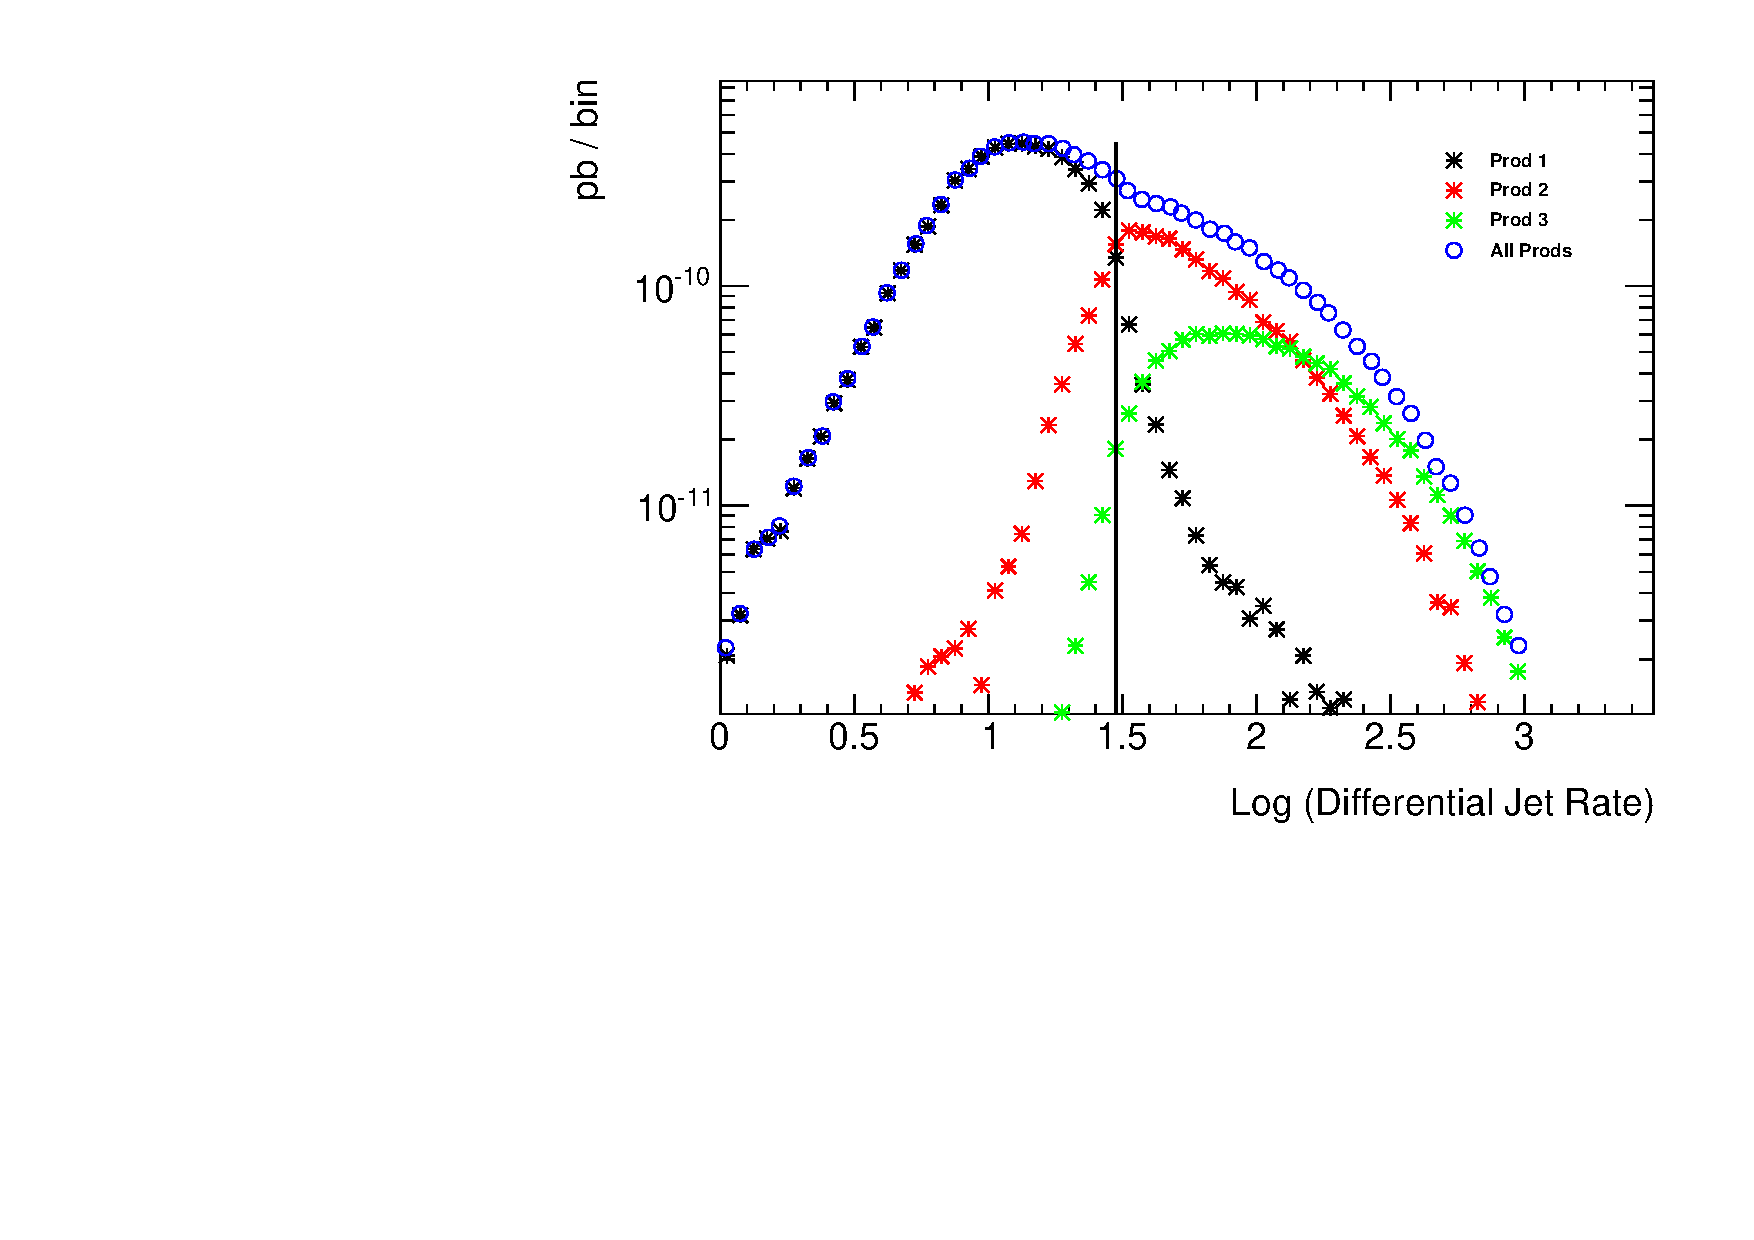
\includegraphics[width=0.48\linewidth]{figures/monojet_appendix/HistoJet1to2_30.pdf}
	}
	\hfill
	\subfloat[$2\rightarrow3$ jets]{%
		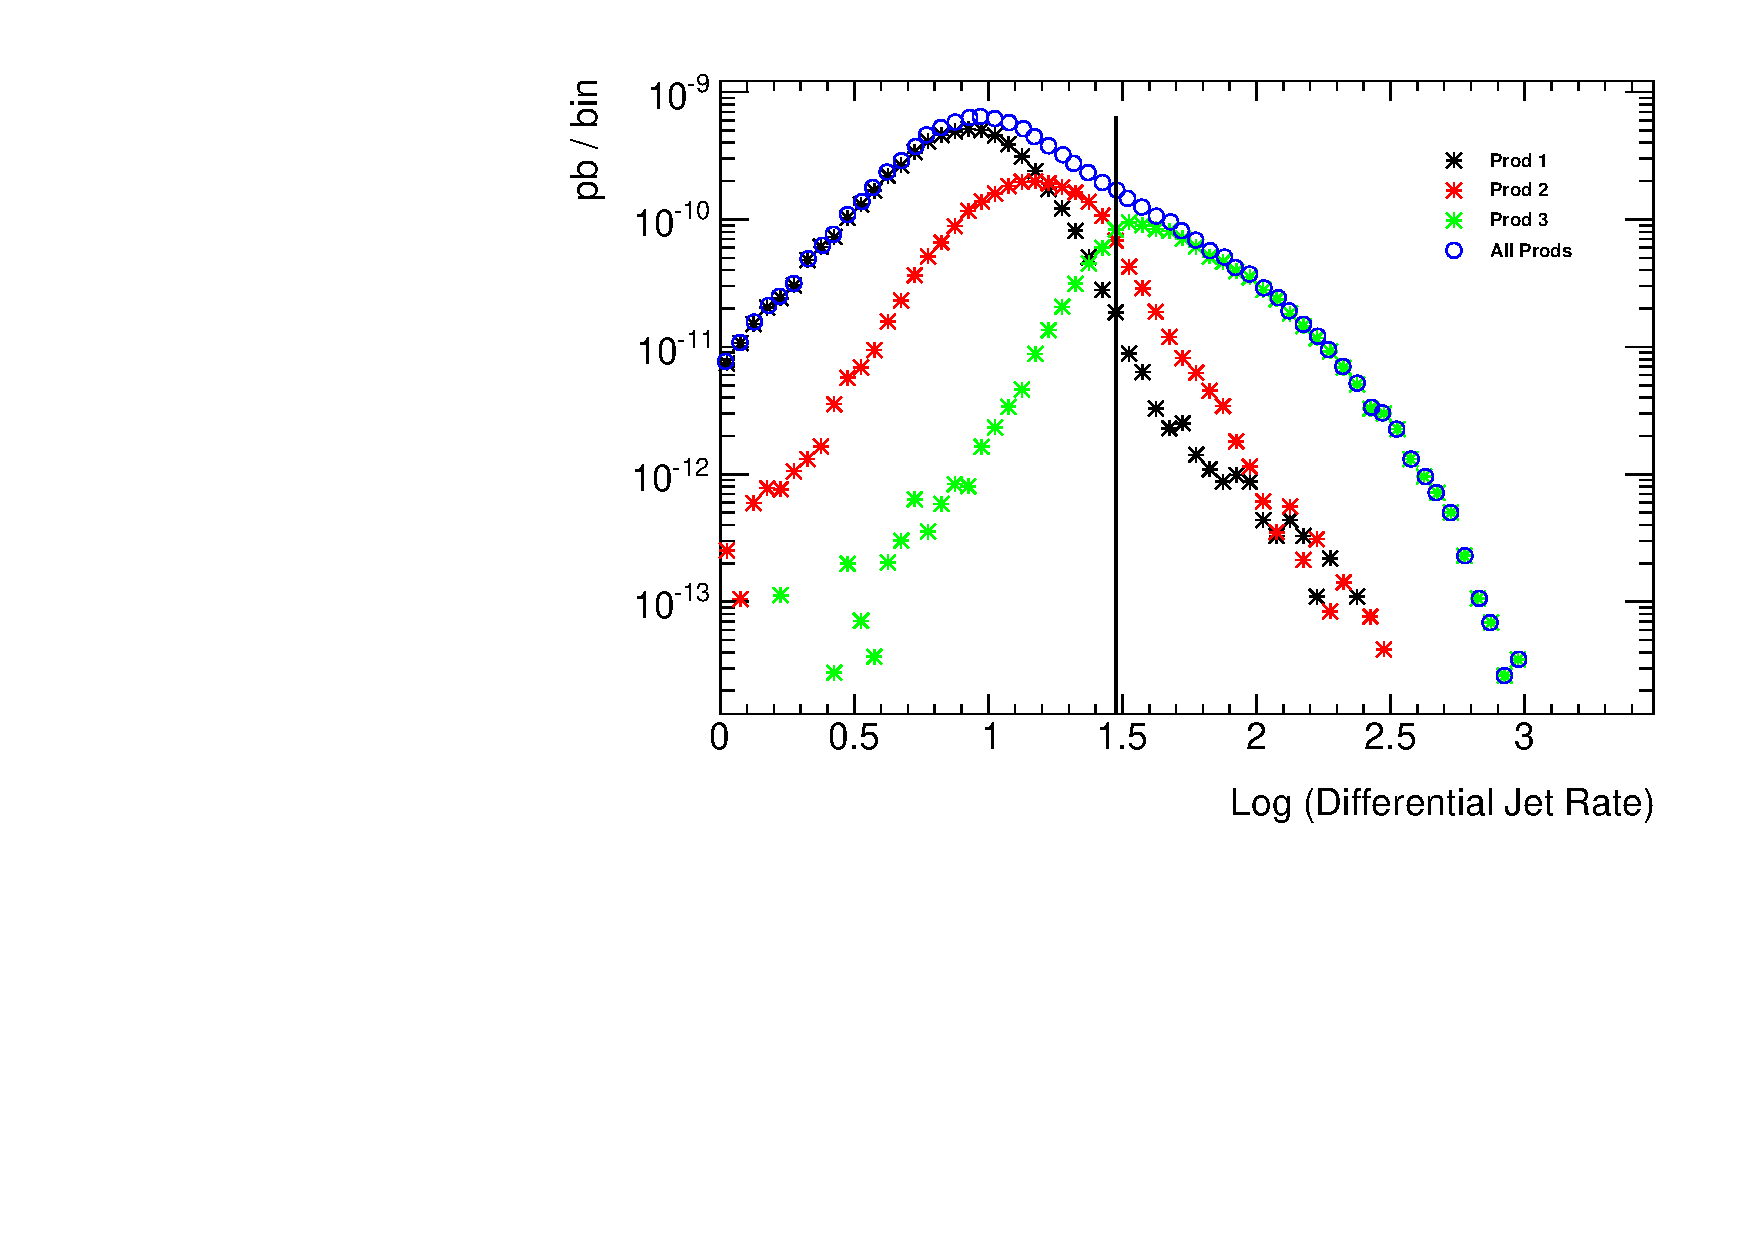
\includegraphics[width=0.48\linewidth]{figures/monojet_appendix/HistoJet2to3_30.pdf}
	}
	\hfill
	\subfloat[$3\rightarrow4$ jets]{%
		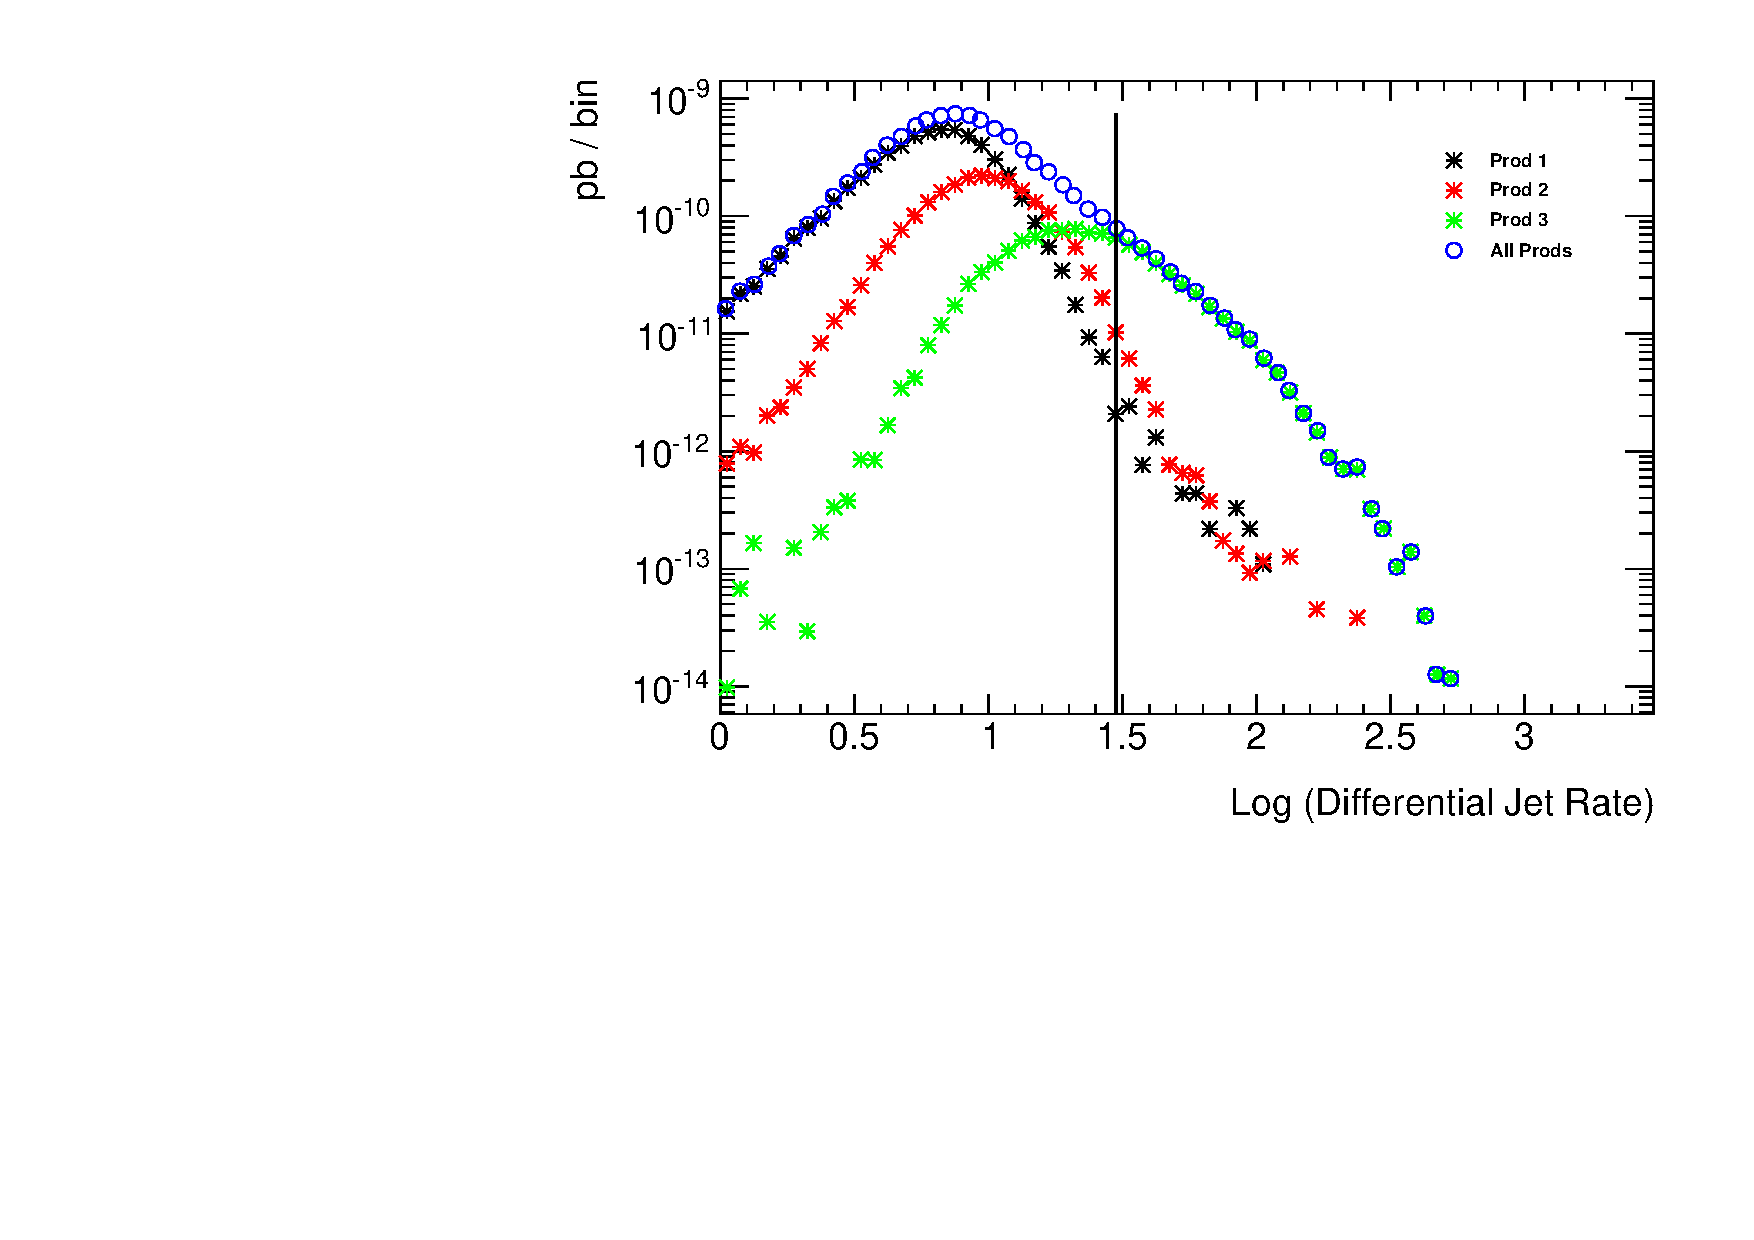
\includegraphics[width=0.48\linewidth]{figures/monojet_appendix/HistoJet3to4_30.pdf}
	}
	\hfill
	\subfloat[$4\rightarrow5$ jets]{%
		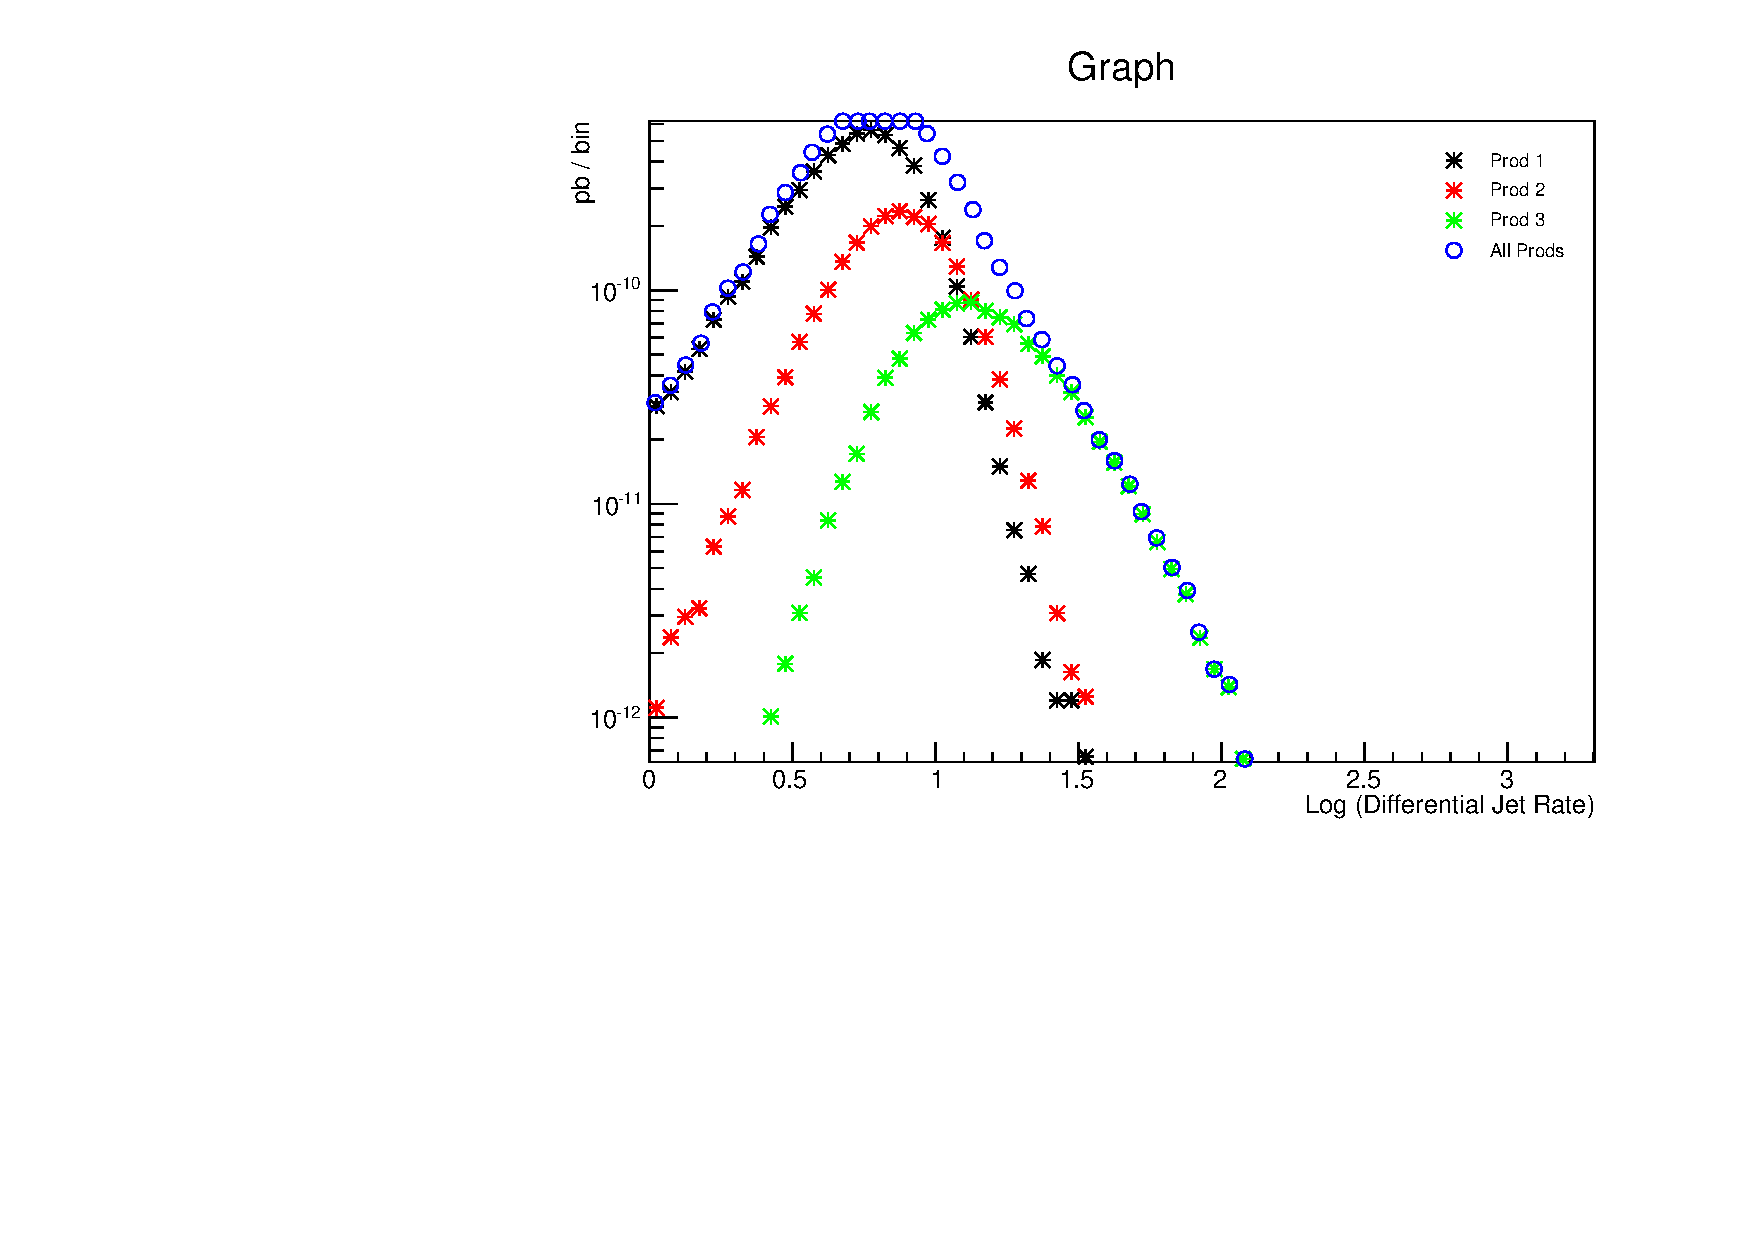
\includegraphics[width=0.48\linewidth]{figures/monojet_appendix/HistoJet4to5_30.pdf}
	}
	\caption{Distributions of differential jet rates $\frac{dN_{i\to j}}{d \log_{10}(k_\textrm{cut})}$ for EFT D5 sample with CKKW-L matching scale at 30\,\gev. The 0-, 1- and 2-parton emission samples are generated separately and indicated in the plots as Prod 1, Prod 2 and Prod 3, respectively. A vertical line is drawn at the matching scale.}
	\label{fig:CKKW_D5_30}
\end{figure}


\begin{figure}[h!]
	\centering  
	\subfloat[$1\rightarrow2$ jets]{%
		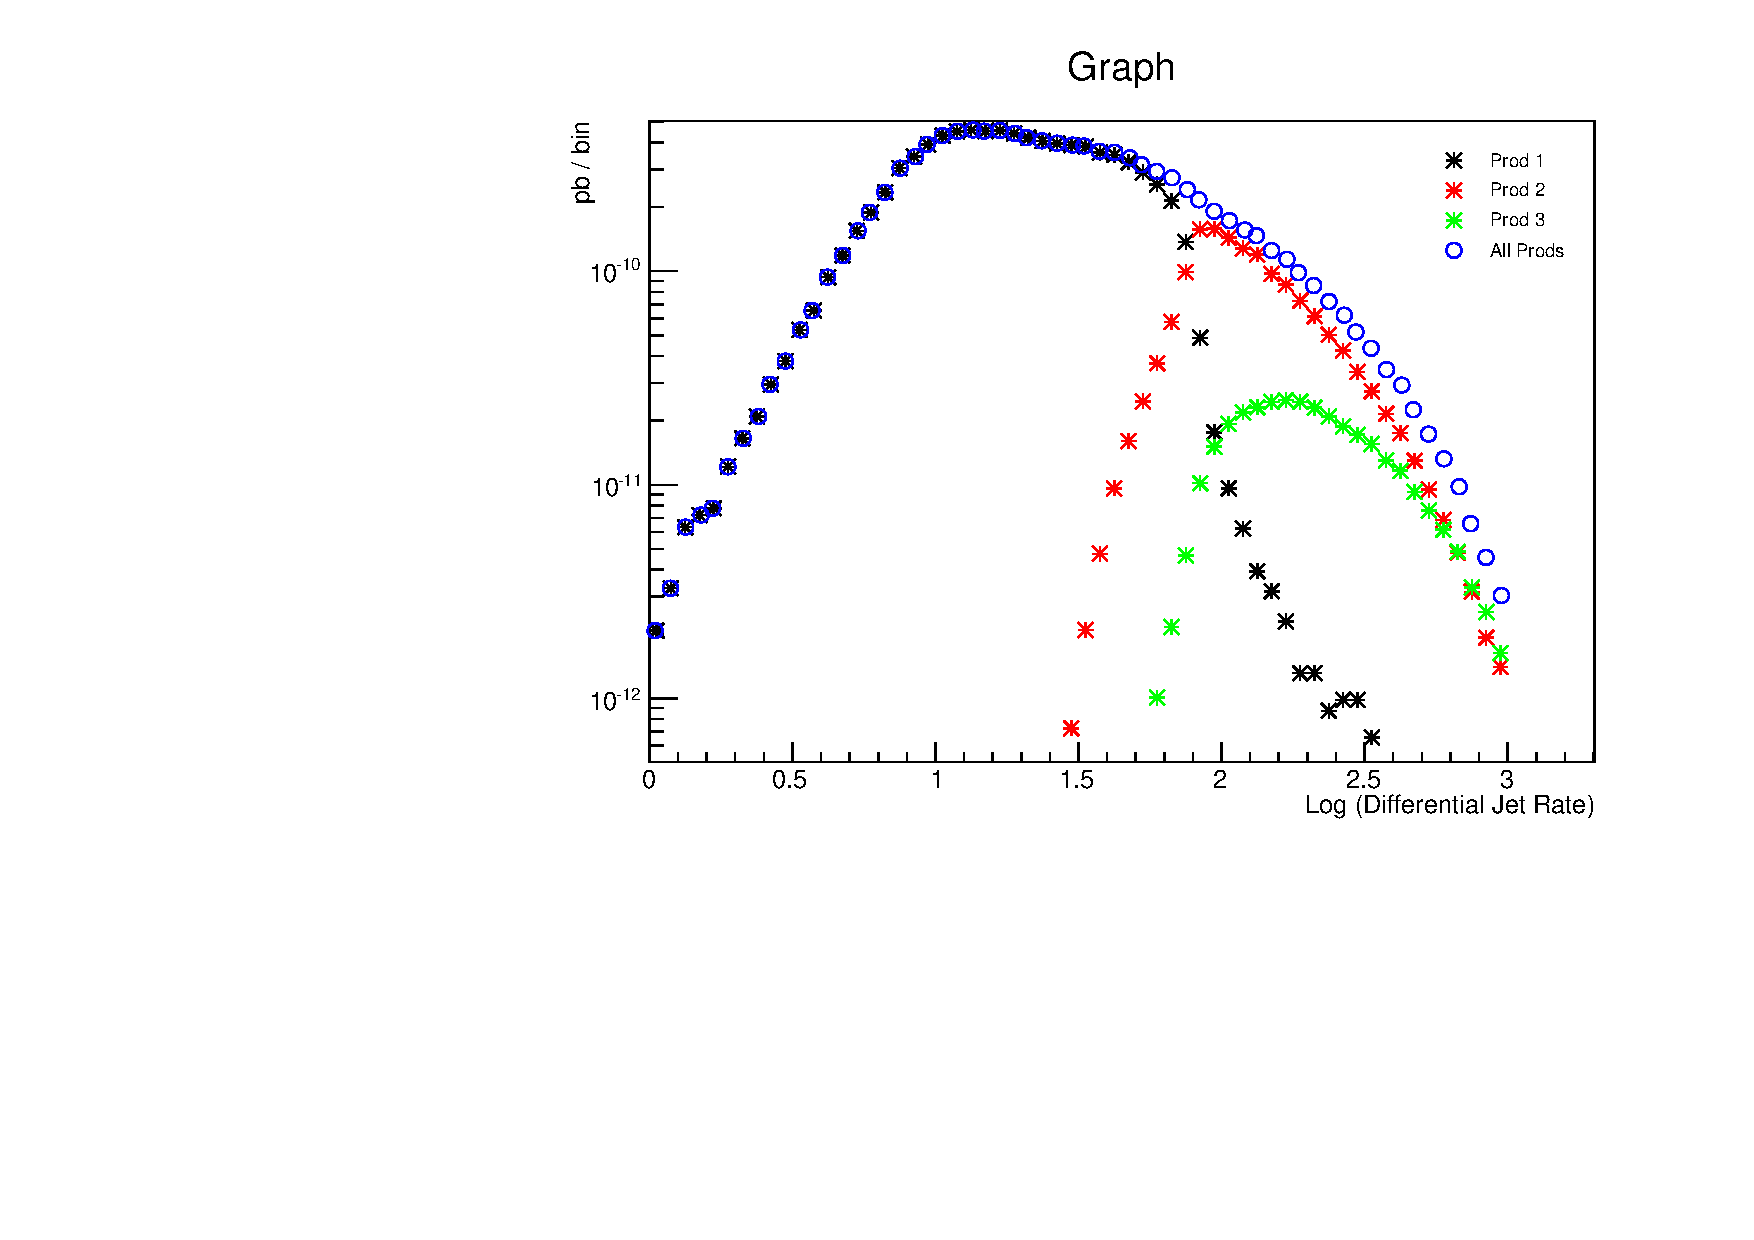
\includegraphics[width=0.48\linewidth]{figures/monojet_appendix/HistoJet1to2_80.pdf}
	}
	\hfill
	\subfloat[$2\rightarrow3$ jets]{%
		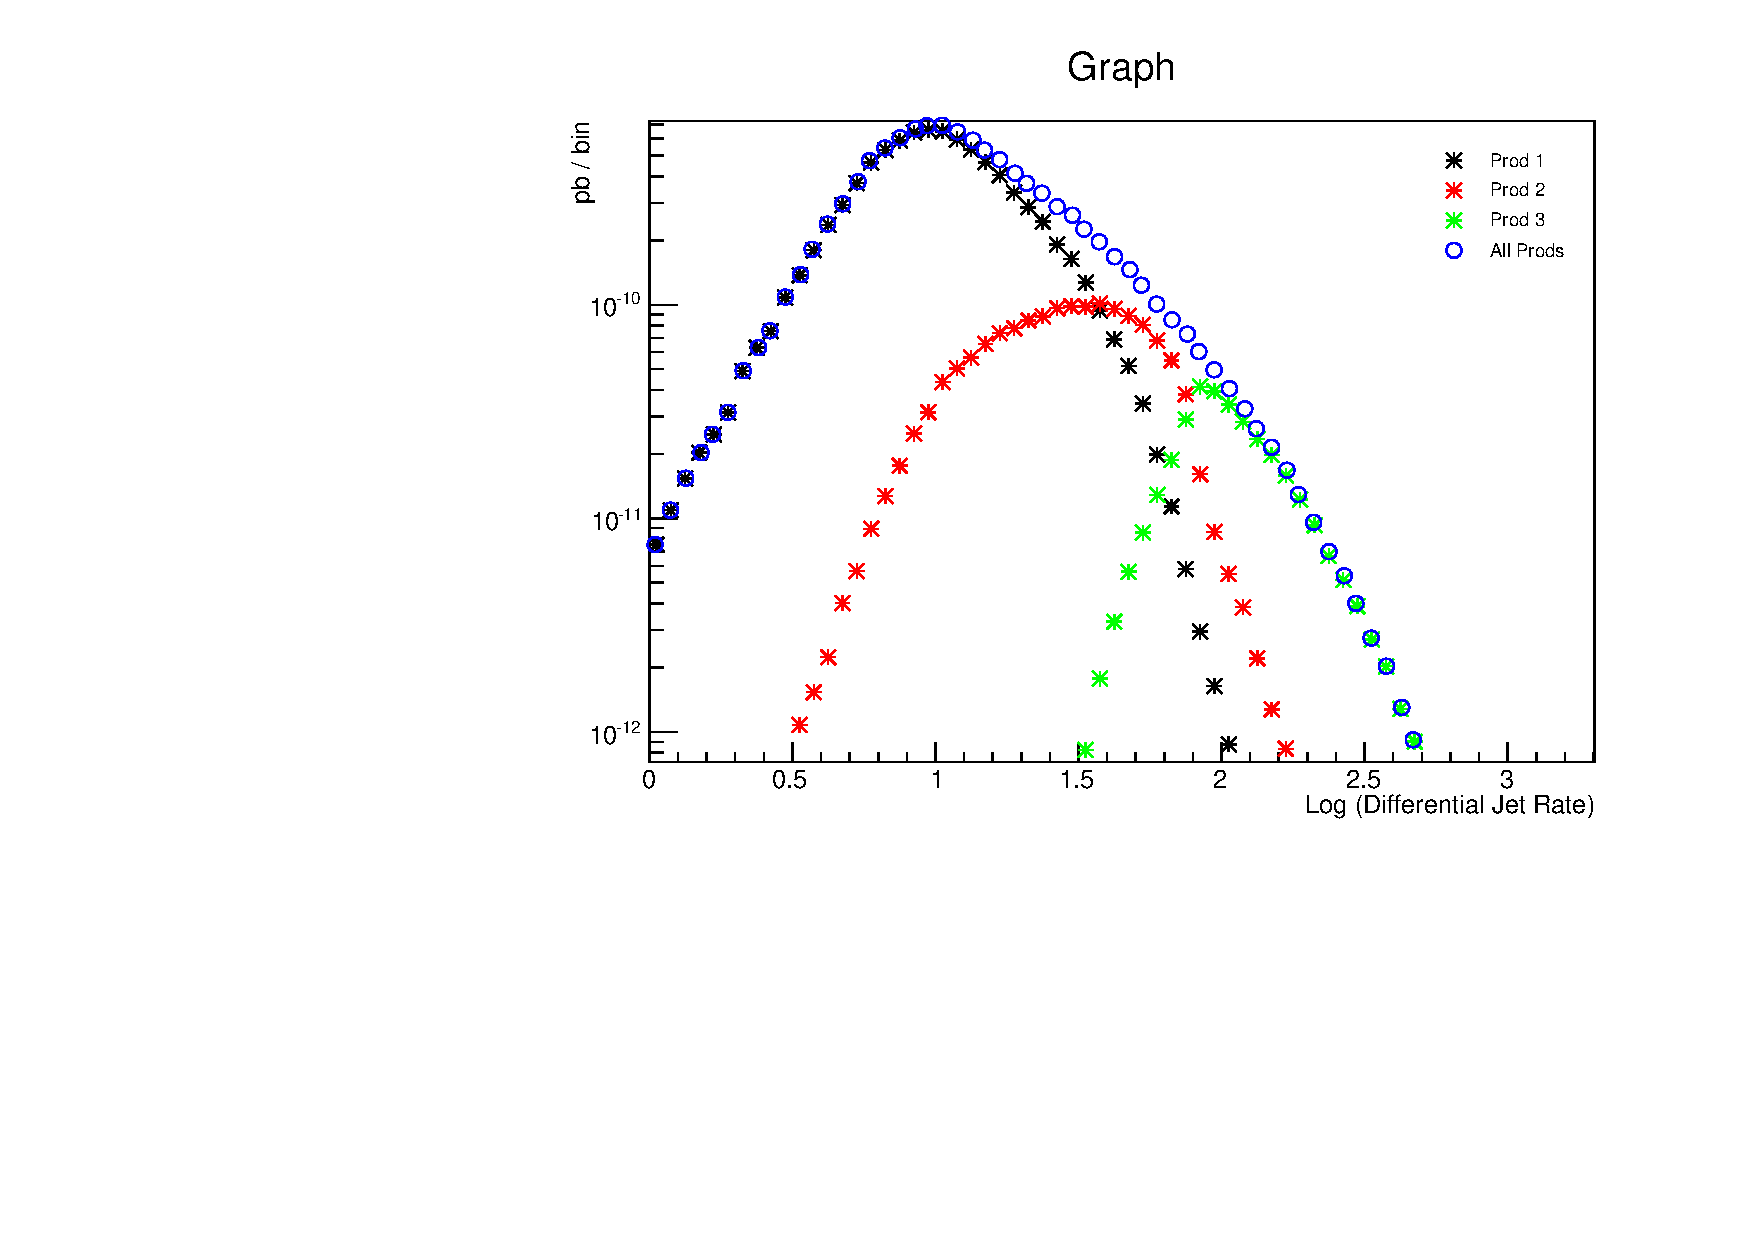
\includegraphics[width=0.48\linewidth]{figures/monojet_appendix/HistoJet2to3_80.pdf}
	}
	\hfill
	\subfloat[$3\rightarrow4$ jets]{%
    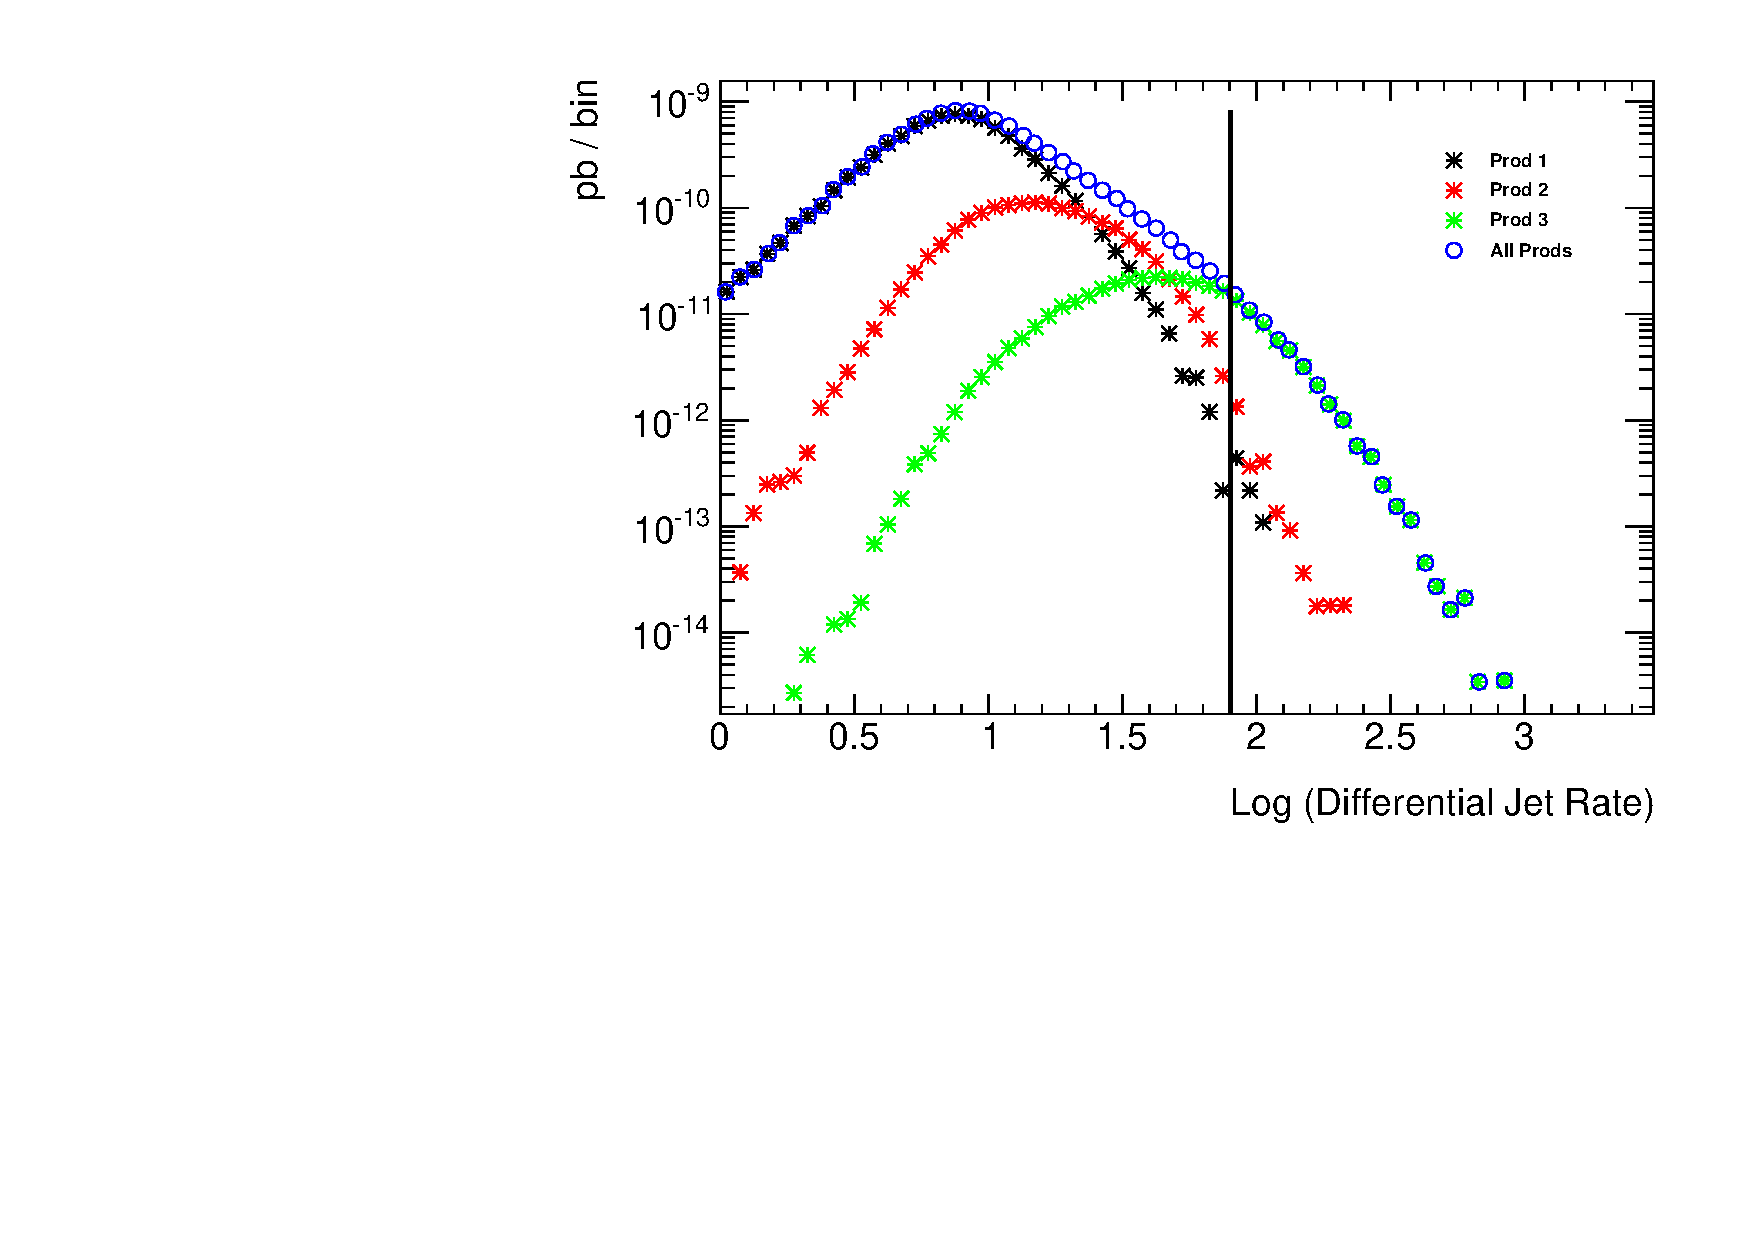
\includegraphics[width=0.48\linewidth]{figures/monojet_appendix/HistoJet3to4_80.pdf}
	}
	\hfill
	\subfloat[$4\rightarrow5$ jets]{%
    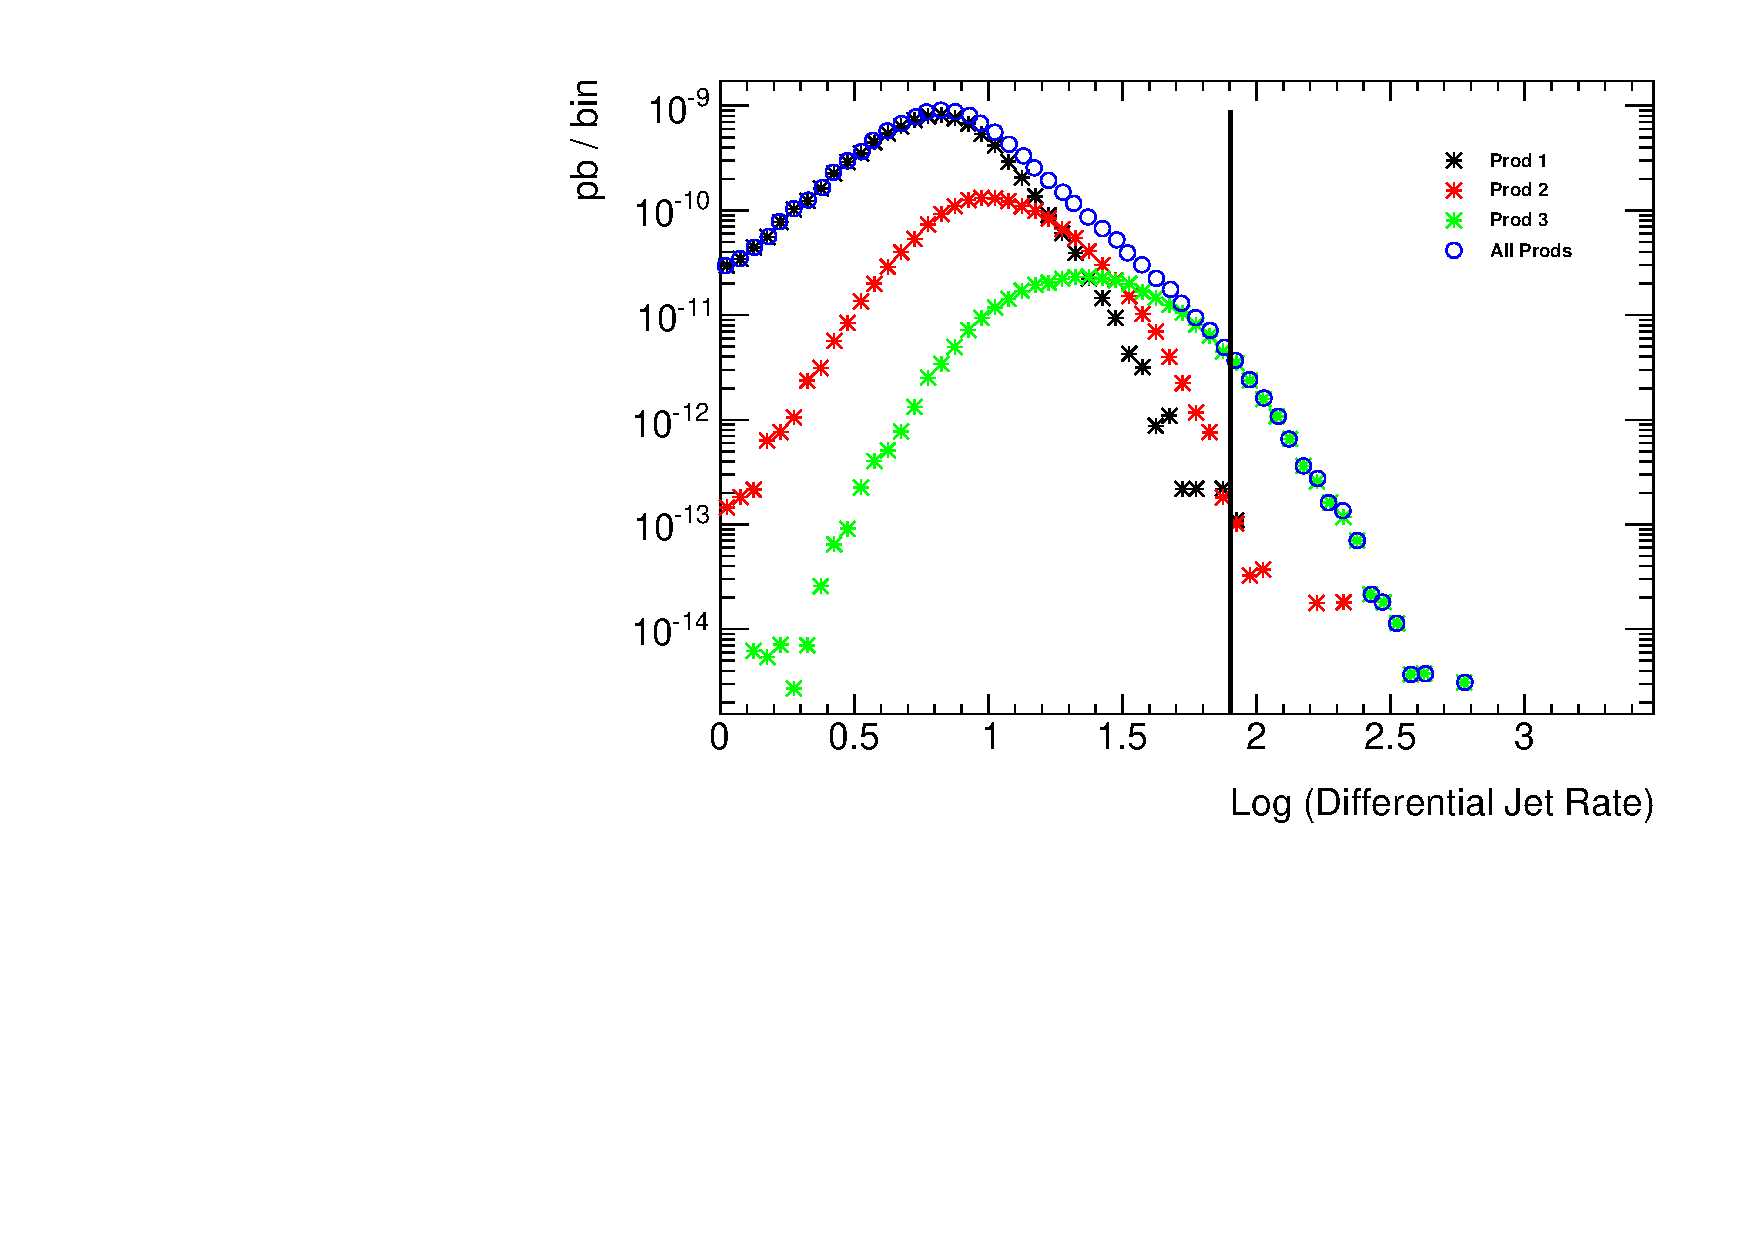
\includegraphics[width=0.48\linewidth]{figures/monojet_appendix/HistoJet4to5_80.pdf}
	}
  \caption{Distributions of differential jet rates $\frac{dN_{i\to j}}{d \log_{10}(k_\textrm{cut})}$ for EFT D5 sample with CKKW-L matching scale at 80\,\gev. The 0-, 1- and 2-parton emission samples are generated separately and indicated in the plots as Prod 1, Prod 2 and Prod 3, respectively. A vertical line is drawn at the matching scale.}
  \label{fig:CKKW_D5_80}
\end{figure}


\begin{figure}[h!]
	\centering  
	\subfloat[$1\rightarrow2$ jets]{%
		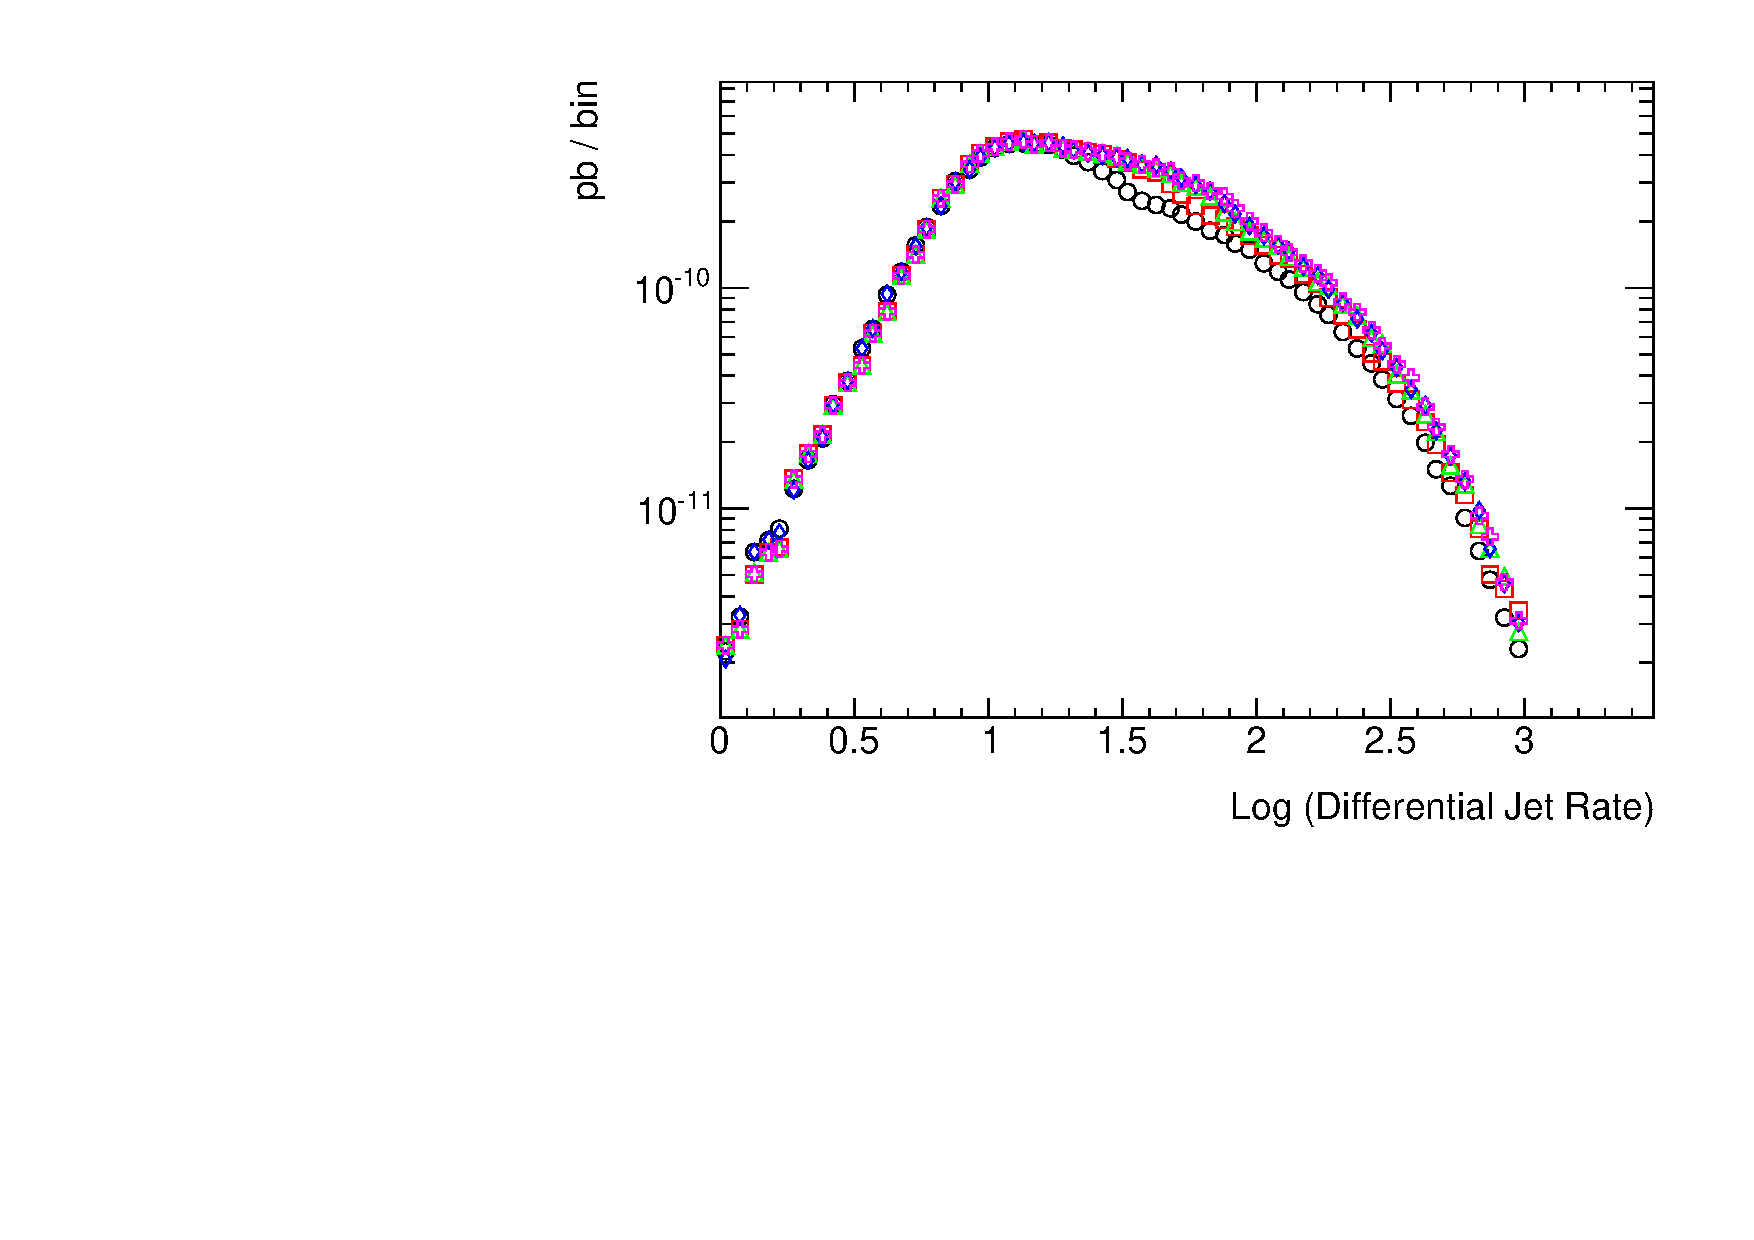
\includegraphics[width=0.48\linewidth]{figures/monojet_appendix/compare_plot_1.pdf}
		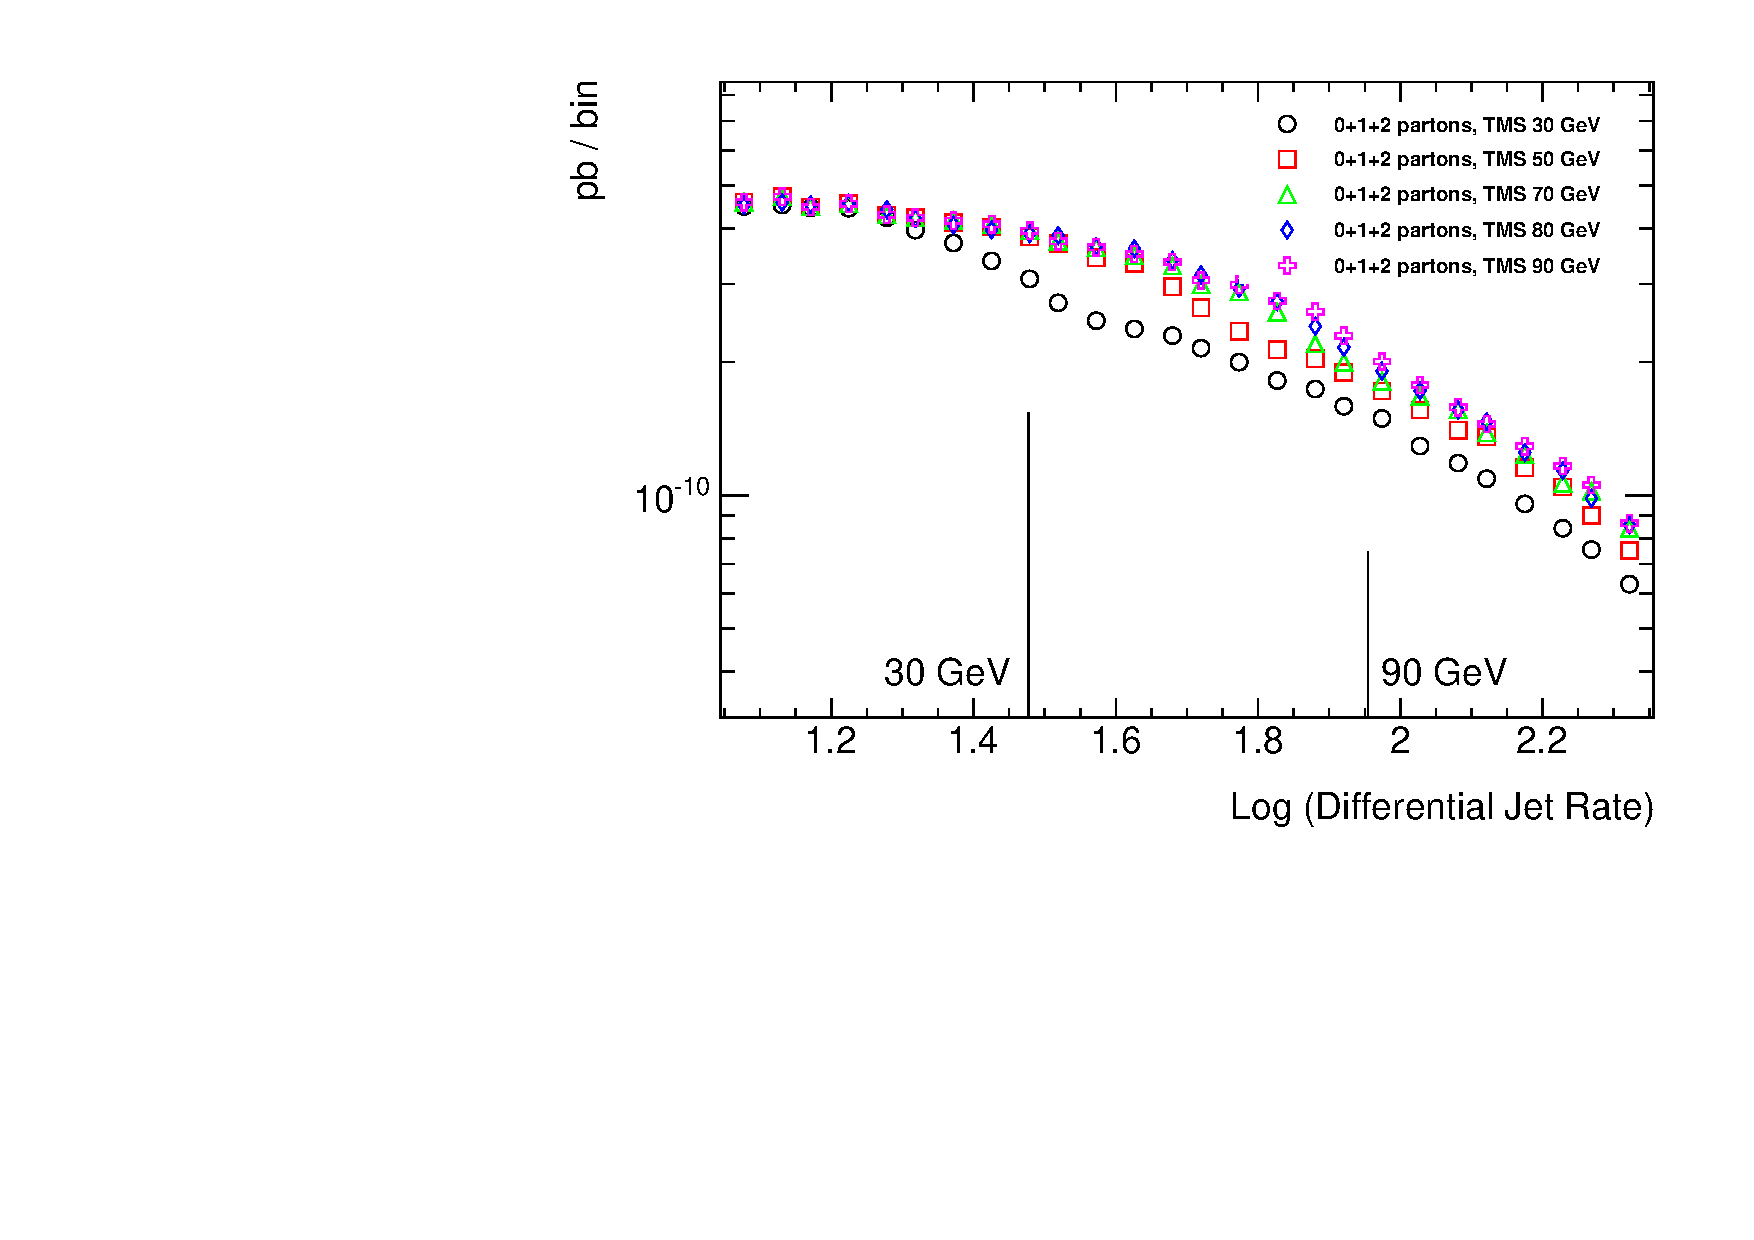
\includegraphics[width=0.48\linewidth]{figures/monojet_appendix/window_plot_1.pdf}
	}
	\hfill
	\subfloat[$2\rightarrow3$ jets]{%
		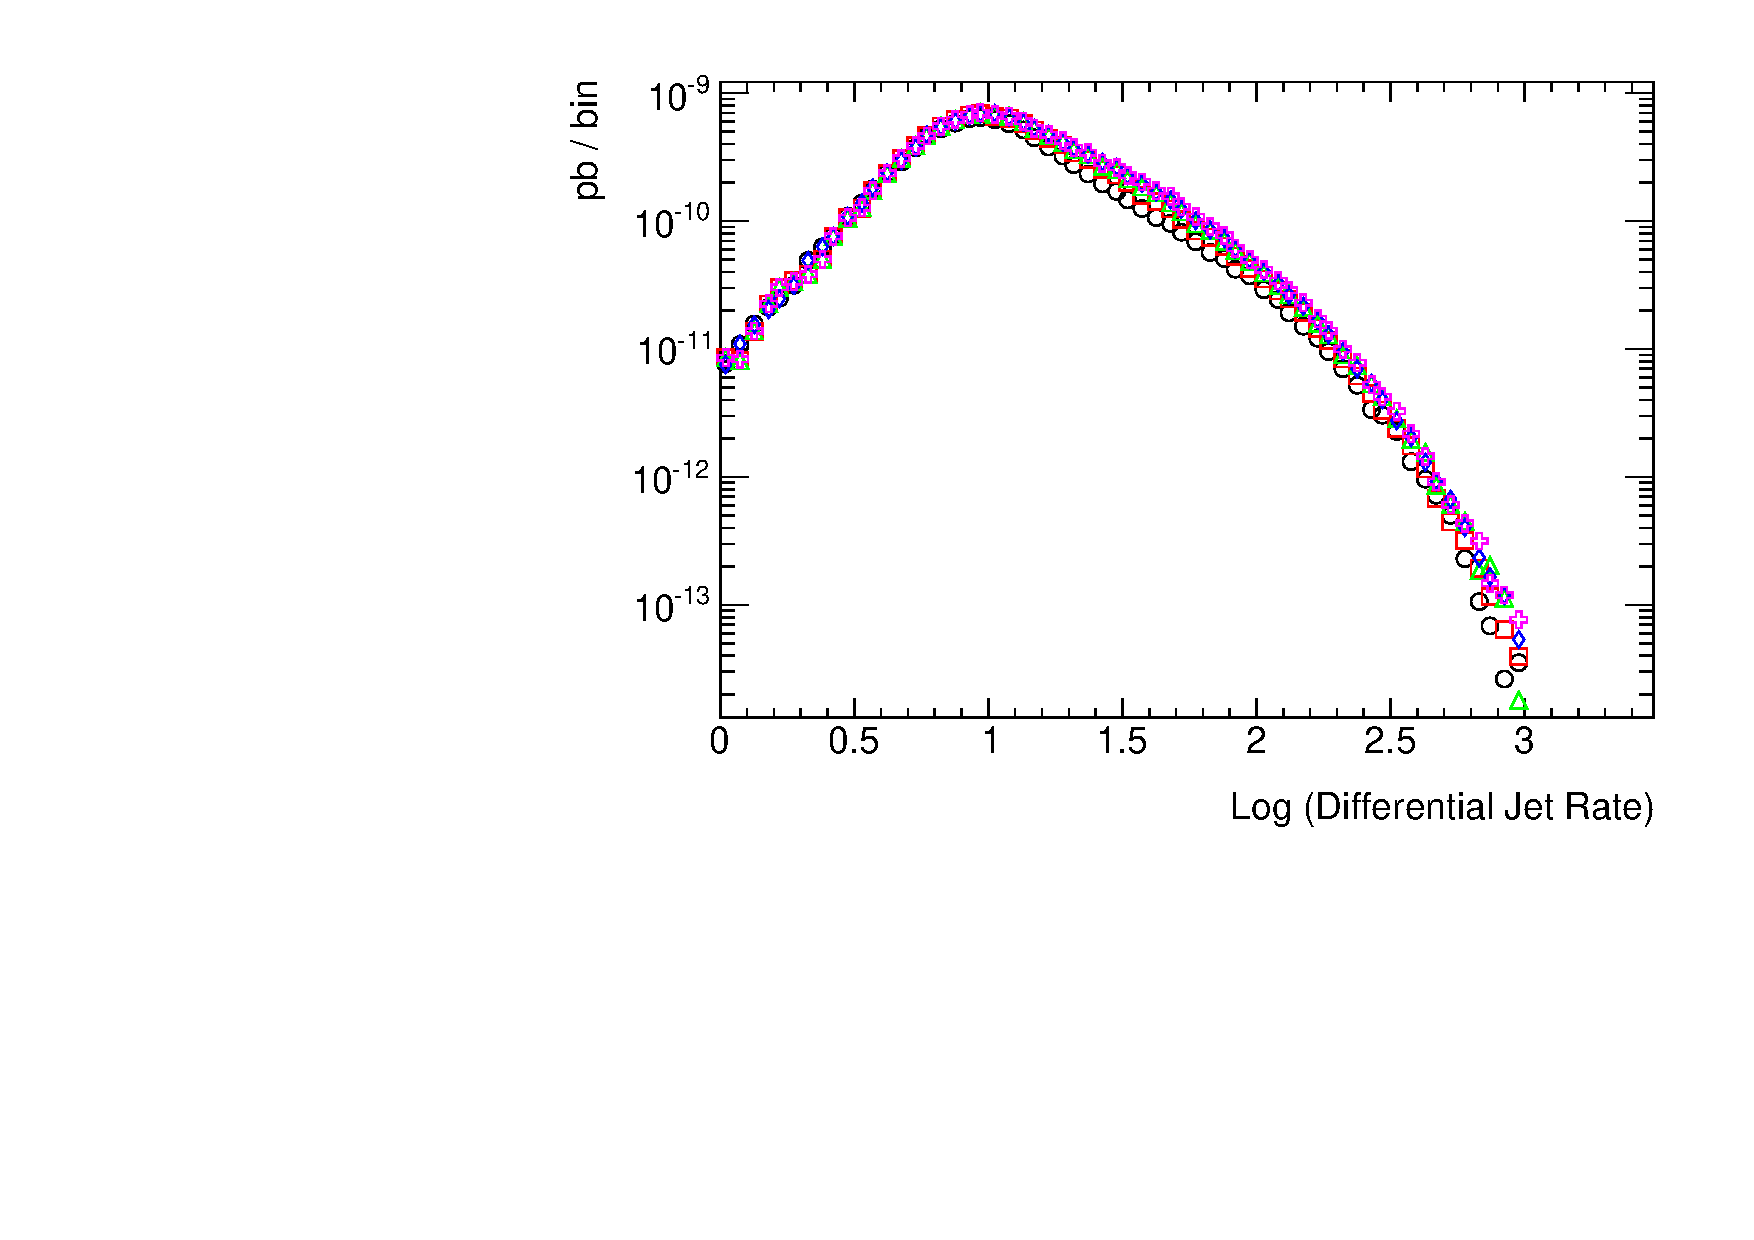
\includegraphics[width=0.48\linewidth]{figures/monojet_appendix/compare_plot_2.pdf}
		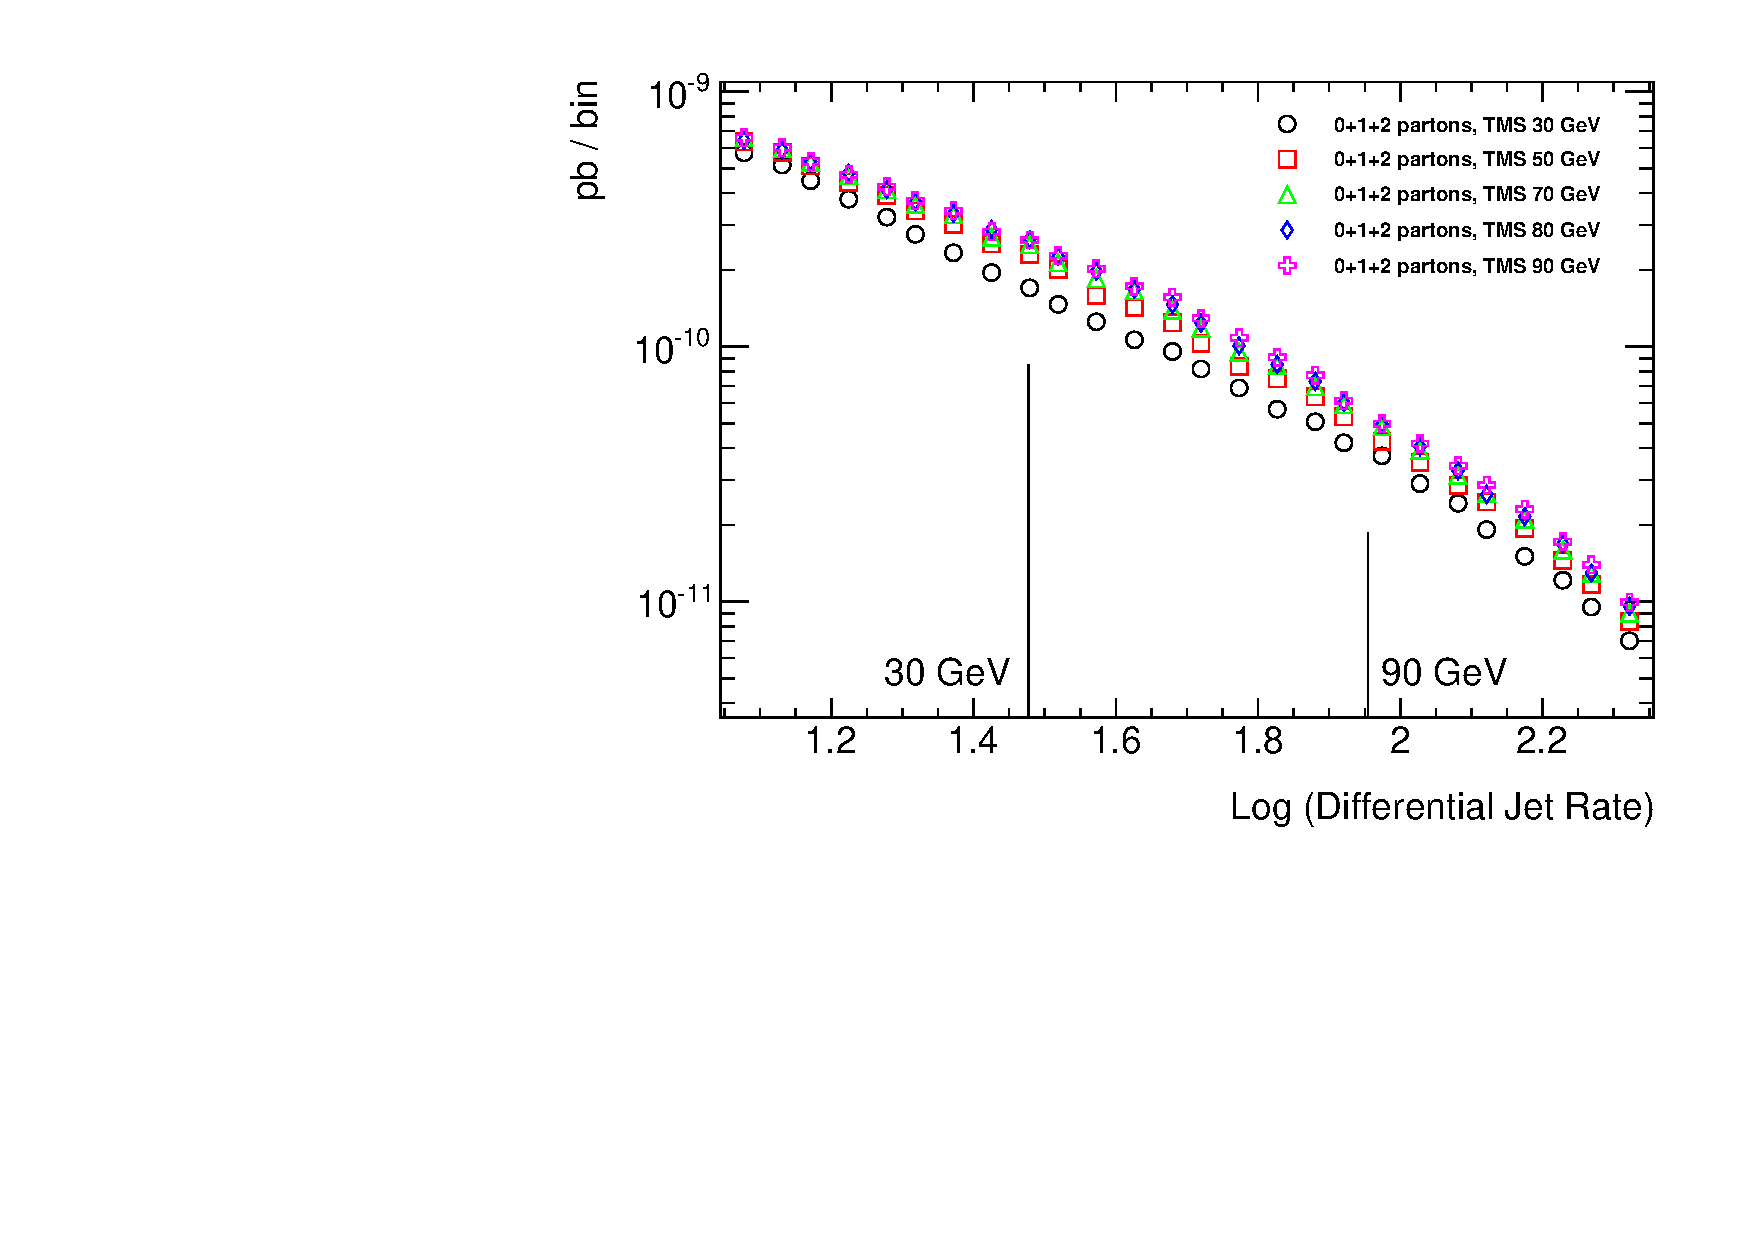
\includegraphics[width=0.48\linewidth]{figures/monojet_appendix/window_plot_2.pdf}
	}
	\hfill
	\subfloat[$3\rightarrow4$ jets]{%
		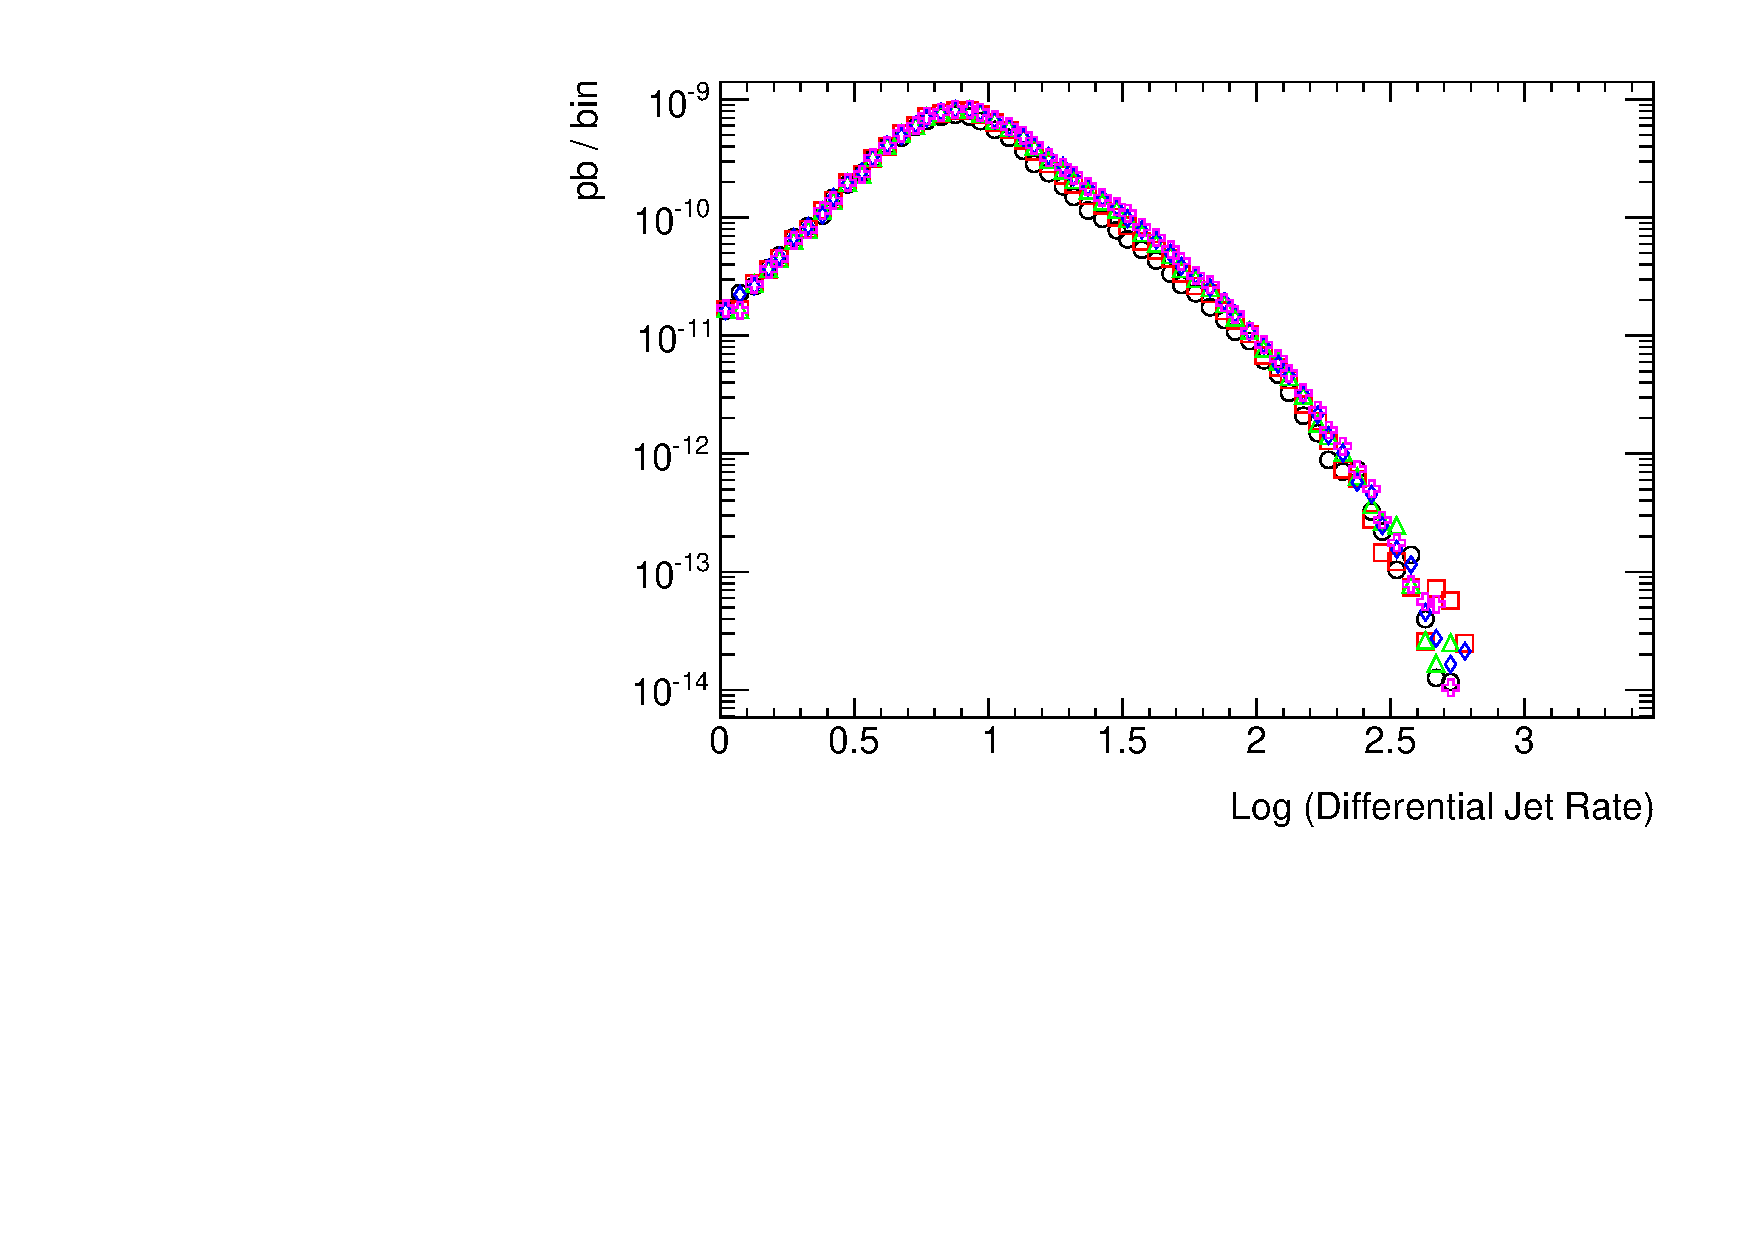
\includegraphics[width=0.48\linewidth]{figures/monojet_appendix/compare_plot_3.pdf}
		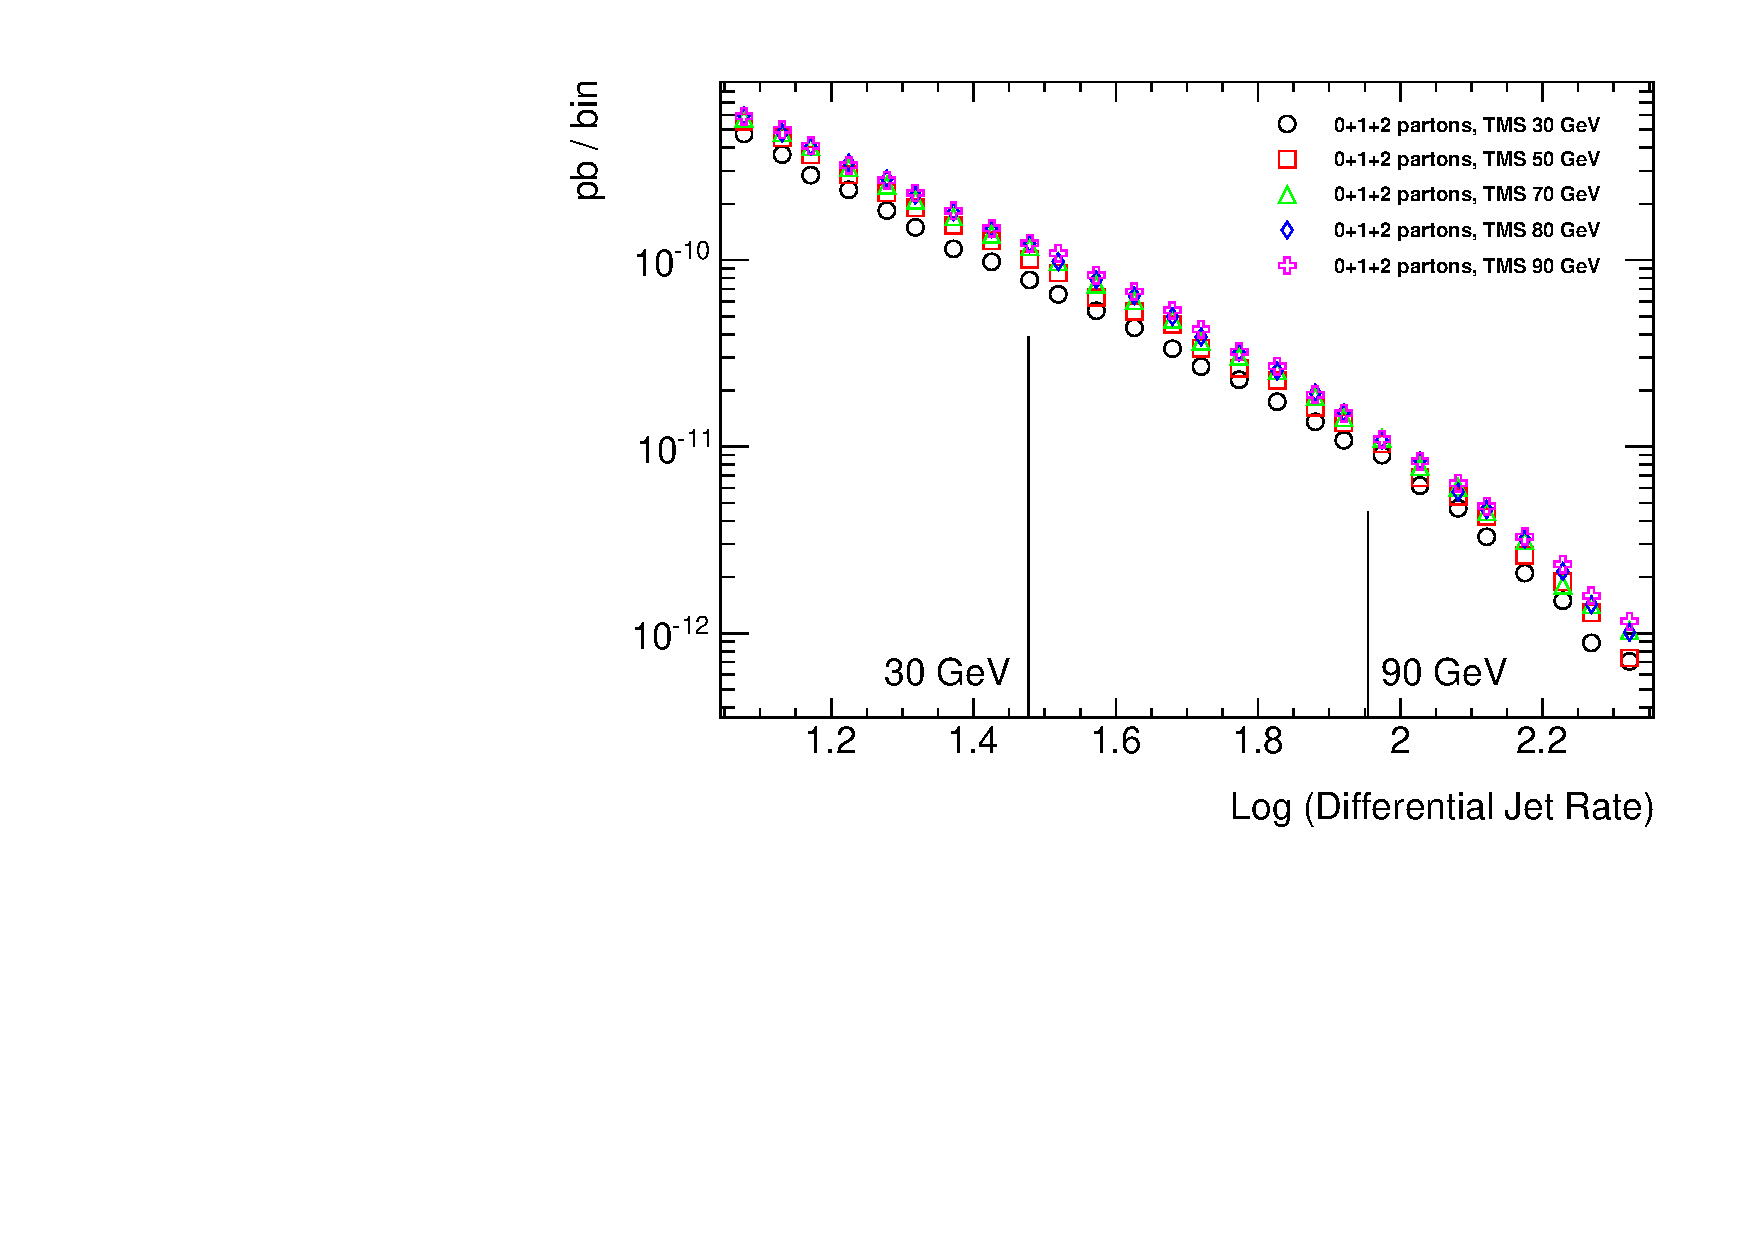
\includegraphics[width=0.48\linewidth]{figures/monojet_appendix/window_plot_3.pdf}
	}
	\hfill
	\subfloat[$4\rightarrow5$ jets]{%
		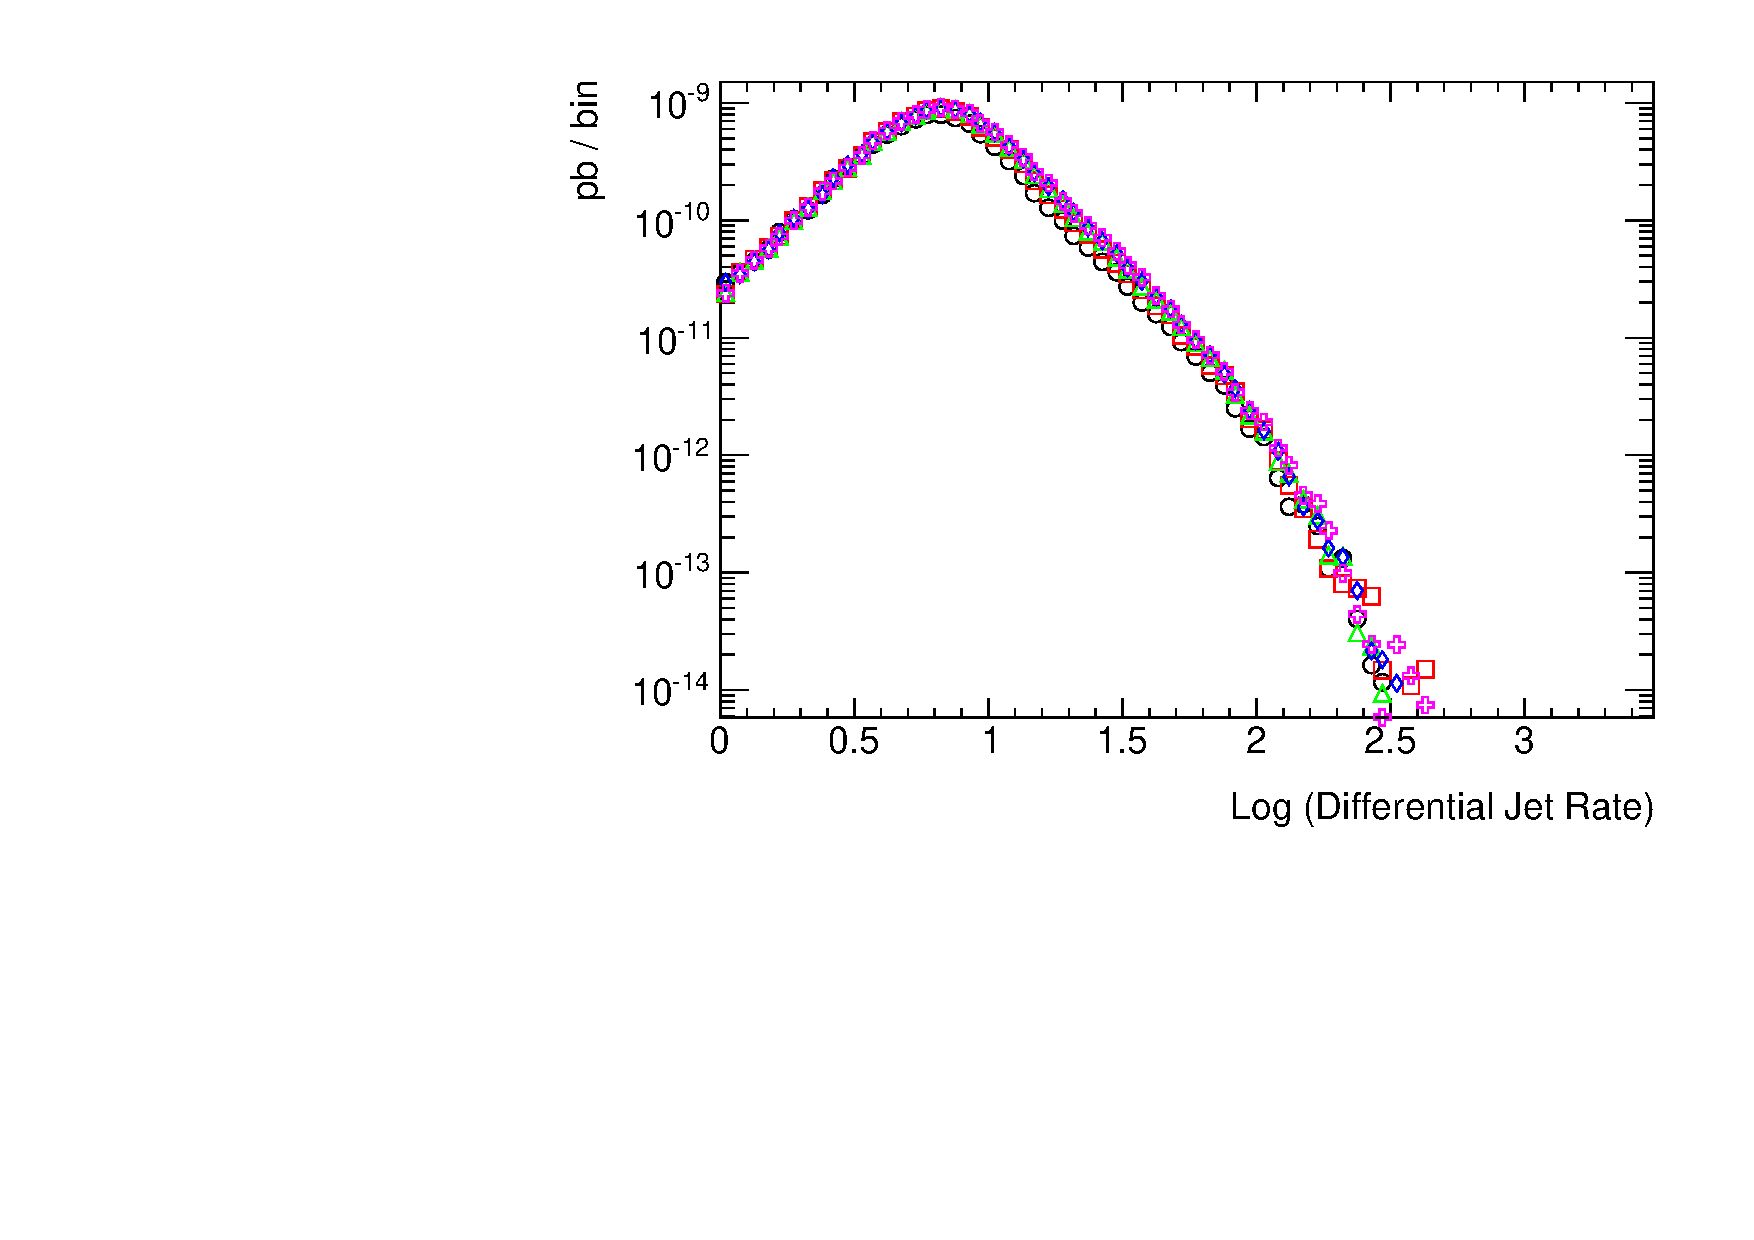
\includegraphics[width=0.48\linewidth]{figures/monojet_appendix/compare_plot_4.pdf}
		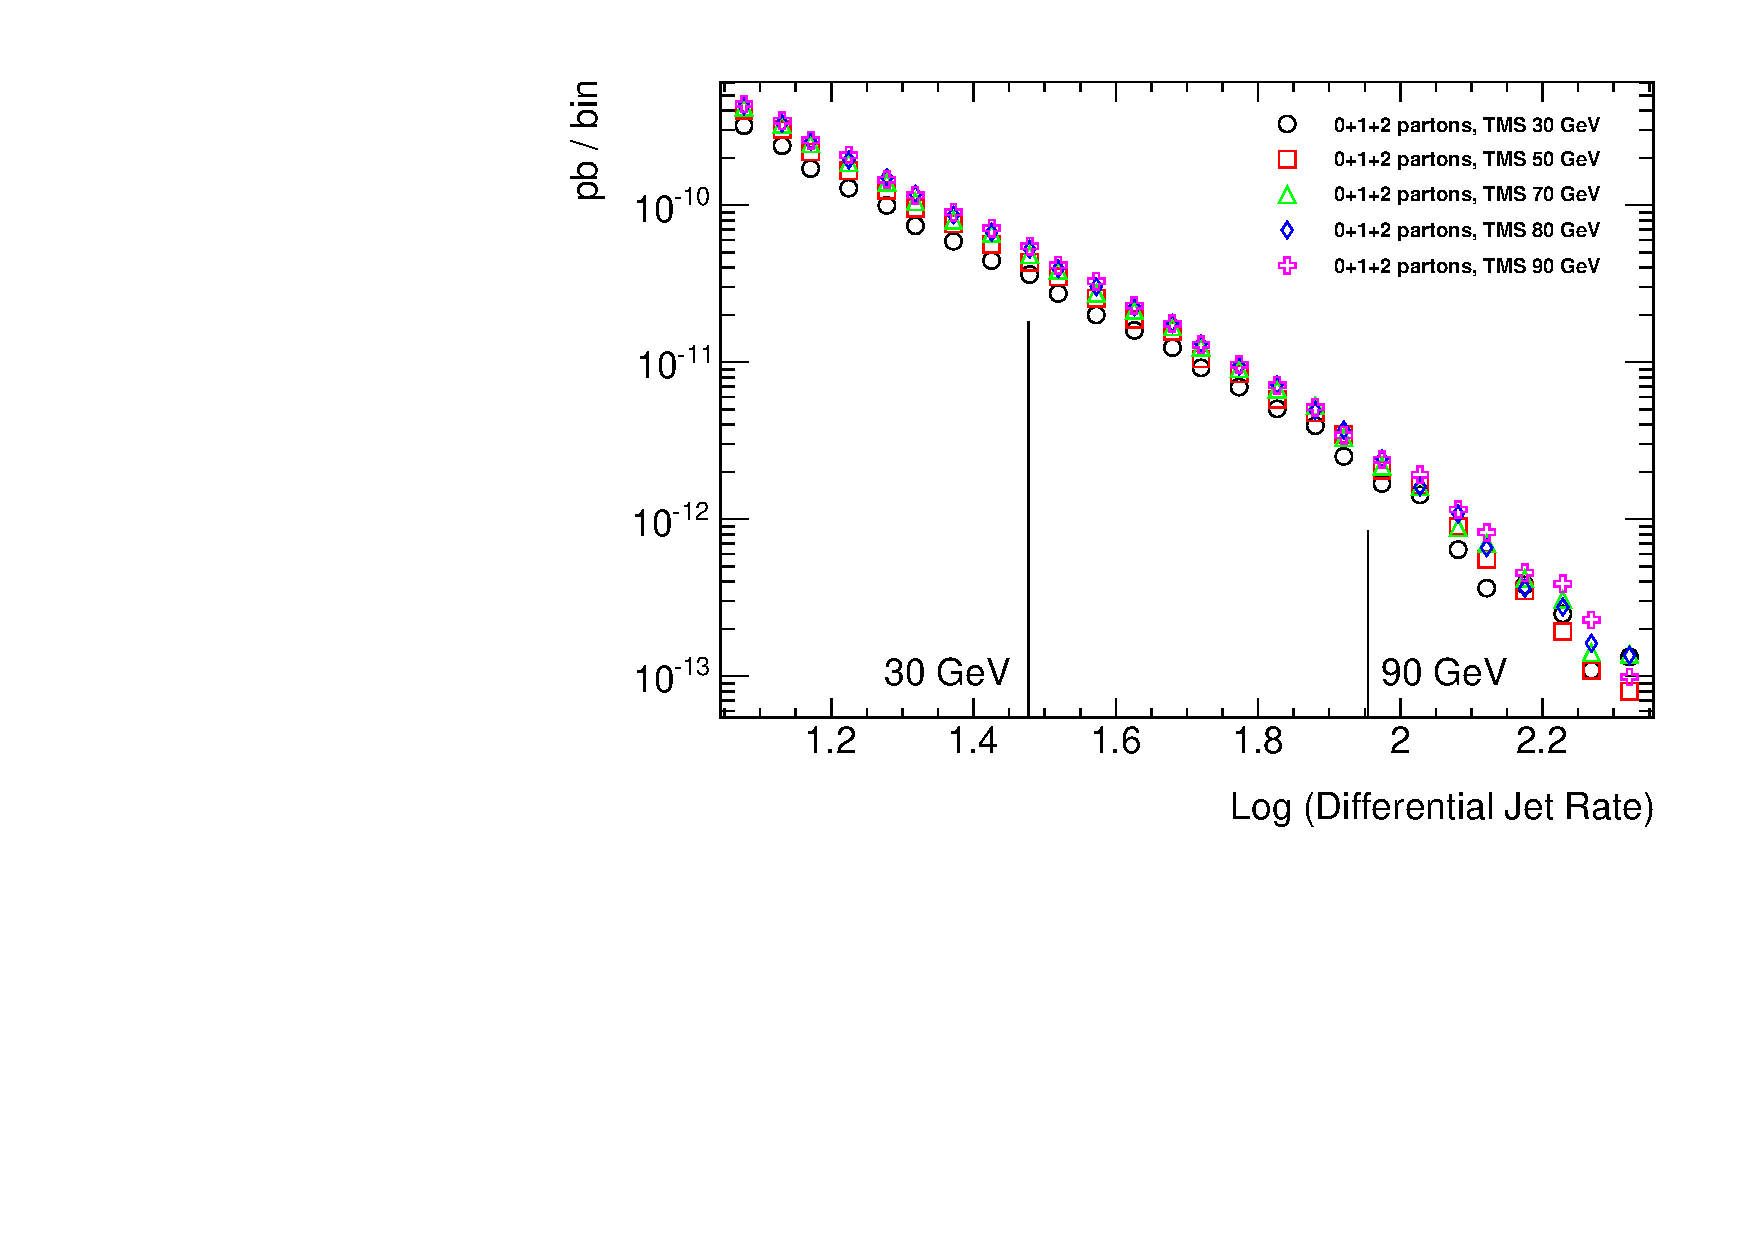
\includegraphics[width=0.48\linewidth]{figures/monojet_appendix/window_plot_4.pdf}
	}
  \caption{Distributions of differential jet rates $\frac{dN_{i\to j}}{d \log_{10}(k_\textrm{cut})}$ for EFT D5 sample with CKKW-L matching scale at 30, 50, 70, 80 and 90\,\gev. A zoom of the region around the matching scale values is shown on right.}
  \label{fig:CKKW_D5_zoom}
\end{figure}




\subsection{Parton emission multiplicity}
\label{sec:monojet_parton_emission}

The prescription for the event generation given in Section\,\ref{sec:match_implementation} starts with the emission of 0 partons and ends with maxim 2 partons in addition. Producing the samples separately allows to investigate the relative composition of the individual samples in various parts of the phase space. Figure\,\ref{fig:Kine_D5_80} shows the \MET distribution of the EFT D5 sample with the matching scale at 80\,\gev. The plot reveals that the 0-parton sample gives the dominant contribution in the region below the matching scale value that rapidly decreases at higher \MET. Assuming the lowest analysis \MET cut in Run-2 mono-jet analyses at 300\,\gev, the generation of the 0-parton emission sample can be safely omitted as it only gives $<1\%$ contribution at $\MET>300\,\gev$. For the 1- and 2-parton emission samples, one can use a generator cut on the leading parton $\pT$, \texttt{ptj1min}, in order to avoid generating low \MET events that are irrelevant for the analysis.

\begin{figure}[h!]
	\centering  
%	\subfloat[Missing transverse momentum]{%
    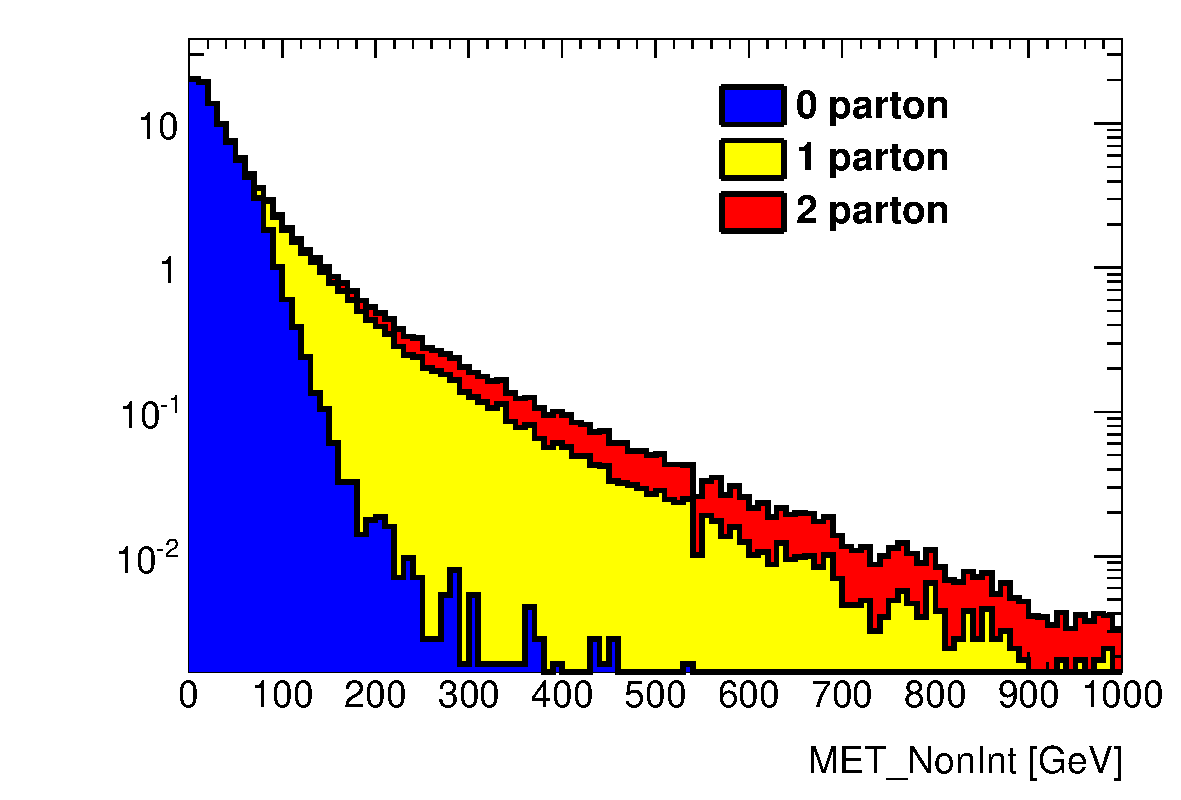
\includegraphics[width=0.8\linewidth]{figures/monojet_appendix/MET_matching80.pdf}
%	}
%	\hfill
%	\subfloat[Transverse momentum of leading jet]{%
%    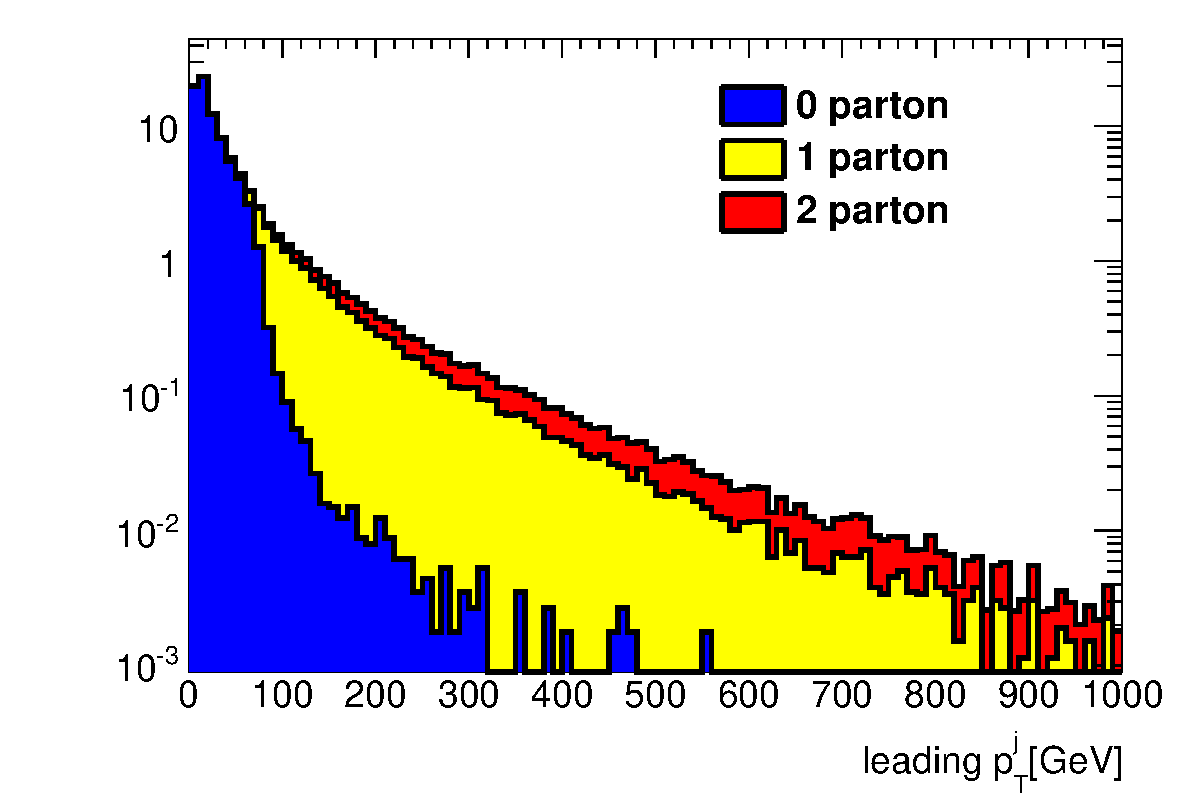
\includegraphics[width=0.48\linewidth]{figures/monojet_appendix/jet1pt_matching80.pdf}
%	}
%	\hfill
%	\subfloat[Transverse momentum of subleading jet]{%
%    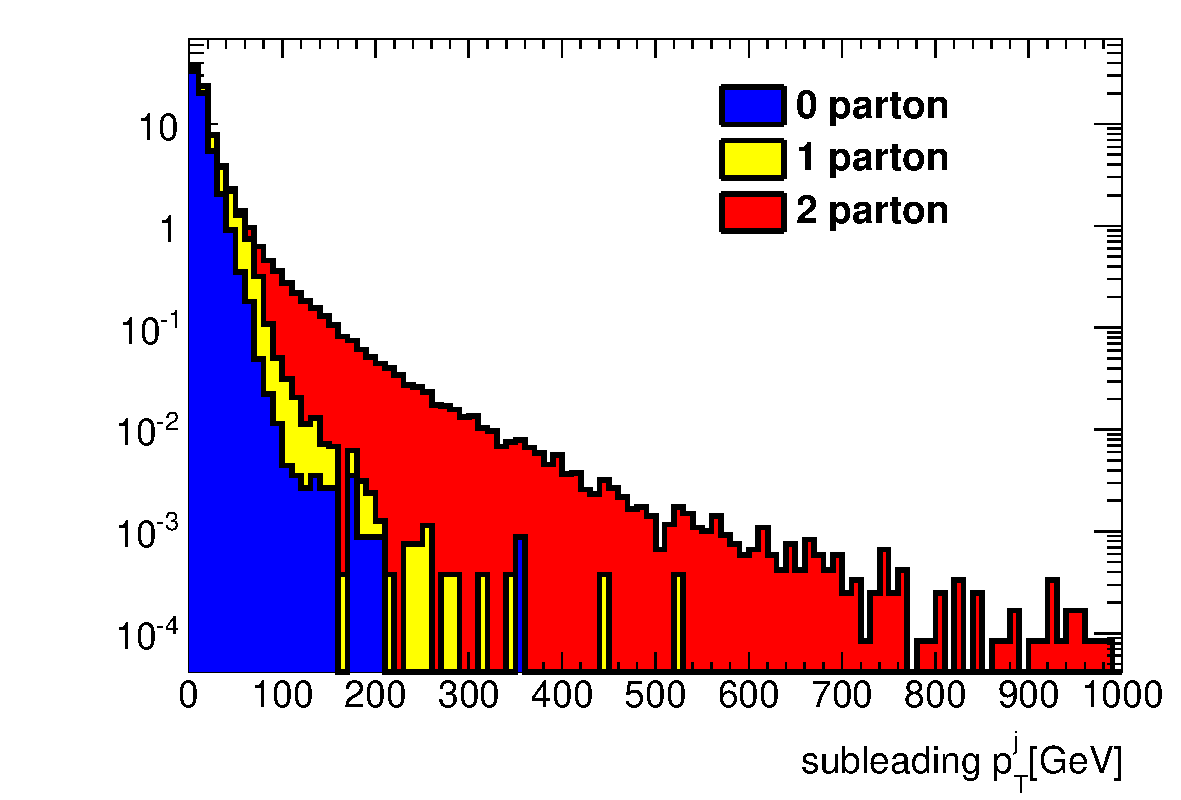
\includegraphics[width=0.48\linewidth]{figures/monojet_appendix/jet2pt_matching80.pdf}
%	}
%	\caption{Kinematics distributions for EFT D5 sample with CKKW matching scale at 80 \gev. 0-, 1- and 2-parton emission cases are generated separately and added together by cross sections. The 0-parton emission case has very limited contribution for missing transverse energy larger than 300 \gev region.}
	\caption{Missing transverse momentum distributions for EFT D5 sample with CKKW-L matching scale at 80\,\gev. Individual contributions from the 0-, 1- and 2-parton emission samples are shown.}
	\label{fig:Kine_D5_80}
\end{figure}



In order to describe the signal kinematics correctly and save time during MC production, the parton emissions will only be generated up to a certain multiplicity. The higher multiplicity samples usually have small enough cross sections and the corresponding parts of the phase space can be sufficiently approximated by parton showering in \pythiaEight.
A dedicated study comparing samples generated with up to 1-, 2-, or 3-parton multiplicities was performed, using again the settings for the CKKW-L $k_t$-merging with the 80\,\gev matching scale and the \texttt{Merging:nJetMax} parameter adjusted accordingly.
Figure\,\ref{fig:RatioKine_D5} shows the \MET distribution of the samples at $\MET>250\,\gev$.

%While there is a $\sim10\%$ difference observed between the samples with up to 1 parton and up to 3 partons at low $\MET$, only marginal difference is seen between the samples generated with up to 2 and 3 partons.

With an event selection requiring \MET and the leading jet \pT being larger than $250\,\gev$ and allowing for up to 4 jets with $\pT>30\,\gev$, the sample generated with up to 1 parton has 17.4\% smaller yield compared to the sample with up to 3 partons, while the yield of the sample with up to 2 partons is only 2.2\% smaller.%At \MET>400\,\gev$, 0+1 parton emission has 16.8\% yield less and 0+1+2 parton emission has 2.4\% less compared to 0+1+2+3 parton emission. With $\MET>600\,\gev$, 0+1 parton emission has 16.5\% yield less and 0+1+2 parton emission has 2.9\% less compared to 0+1+2+3 parton emission. The same numbers hold if a symmetric cut is added on leading jet transverse momentum.
This justifies it is sufficient to produce samples with up to 2 parton emissions only at the generator level and ignore generating higher parton emissions.


\begin{figure}[h!]
	\centering  
	\subfloat[No jet multiplicity cut]{%
		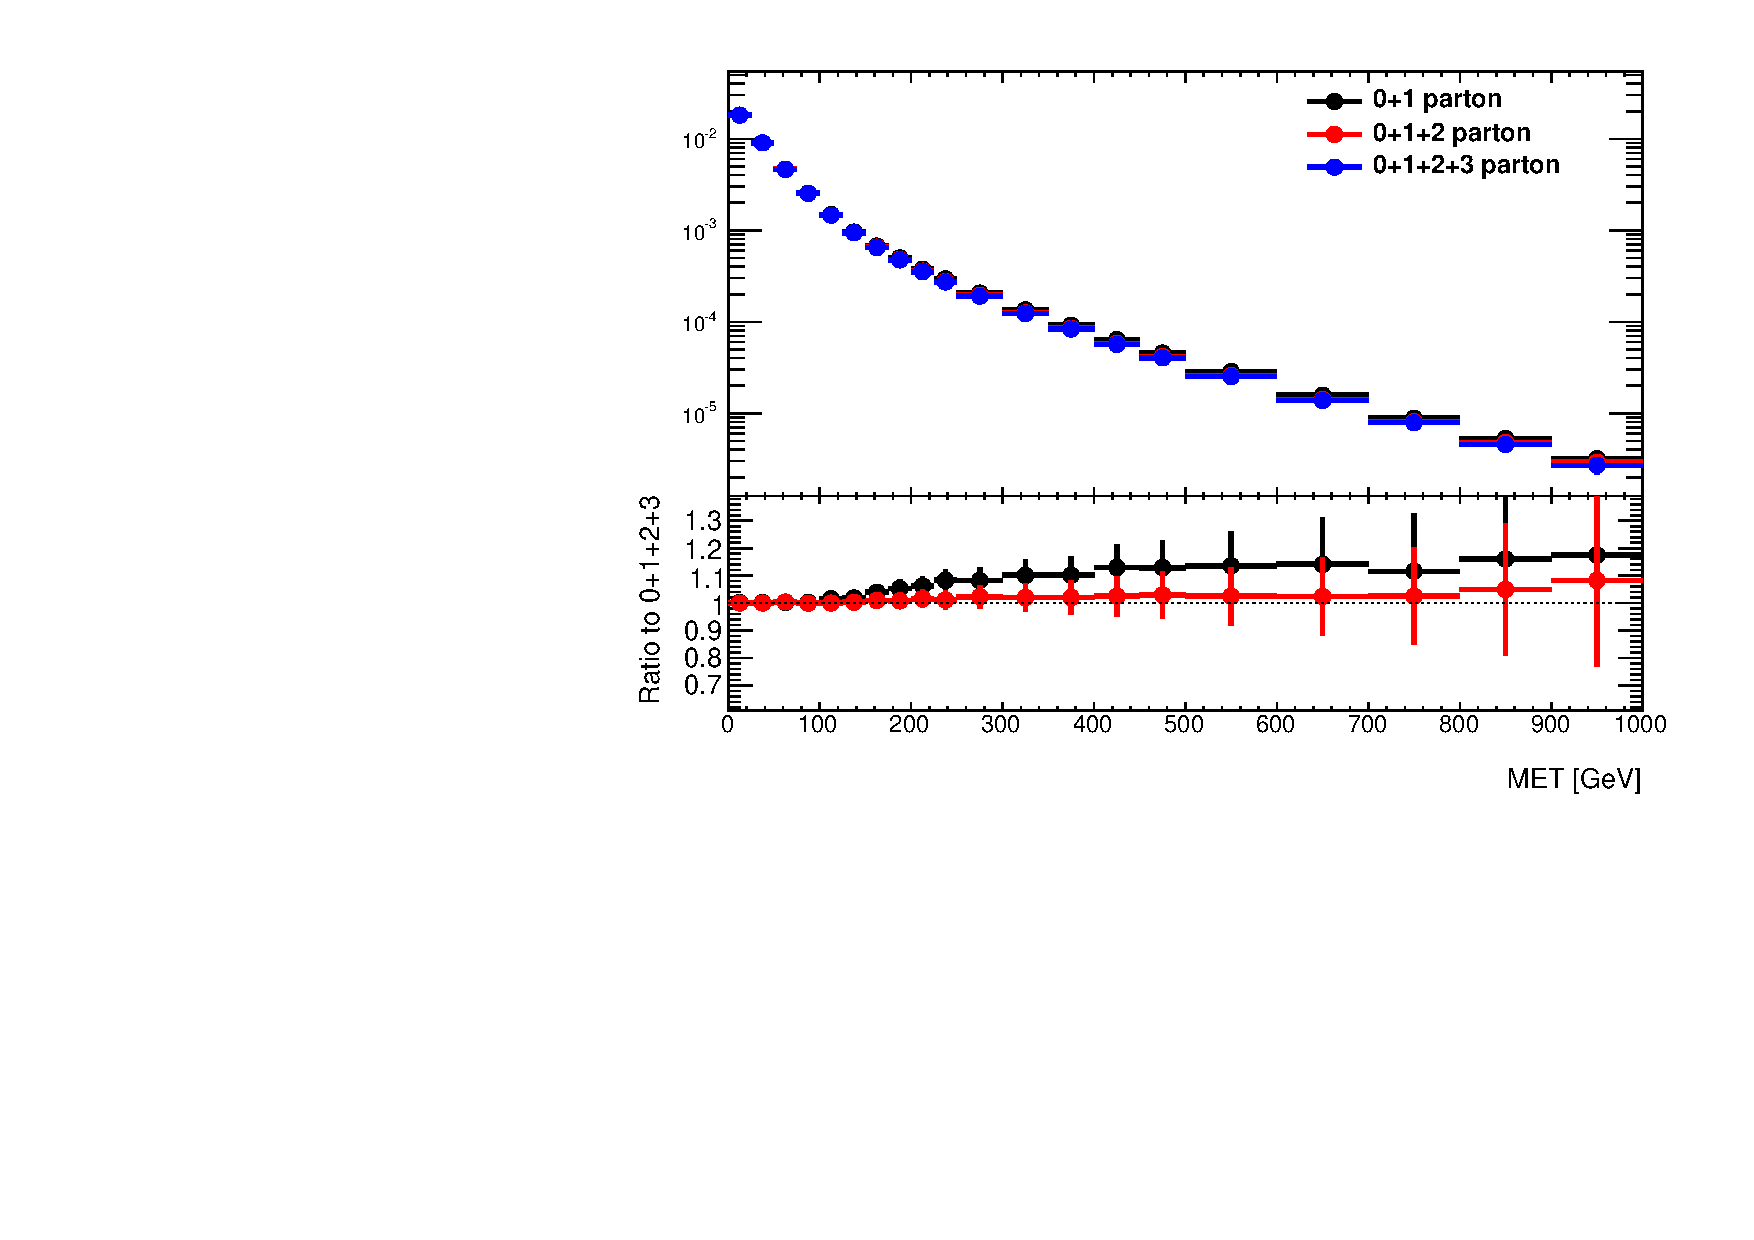
\includegraphics[width=0.48\linewidth]{figures/monojet_appendix/h_MET.pdf}
	}
	\hfill
	\subfloat[$N_{\text{jet}}\leqslant$3]{%
		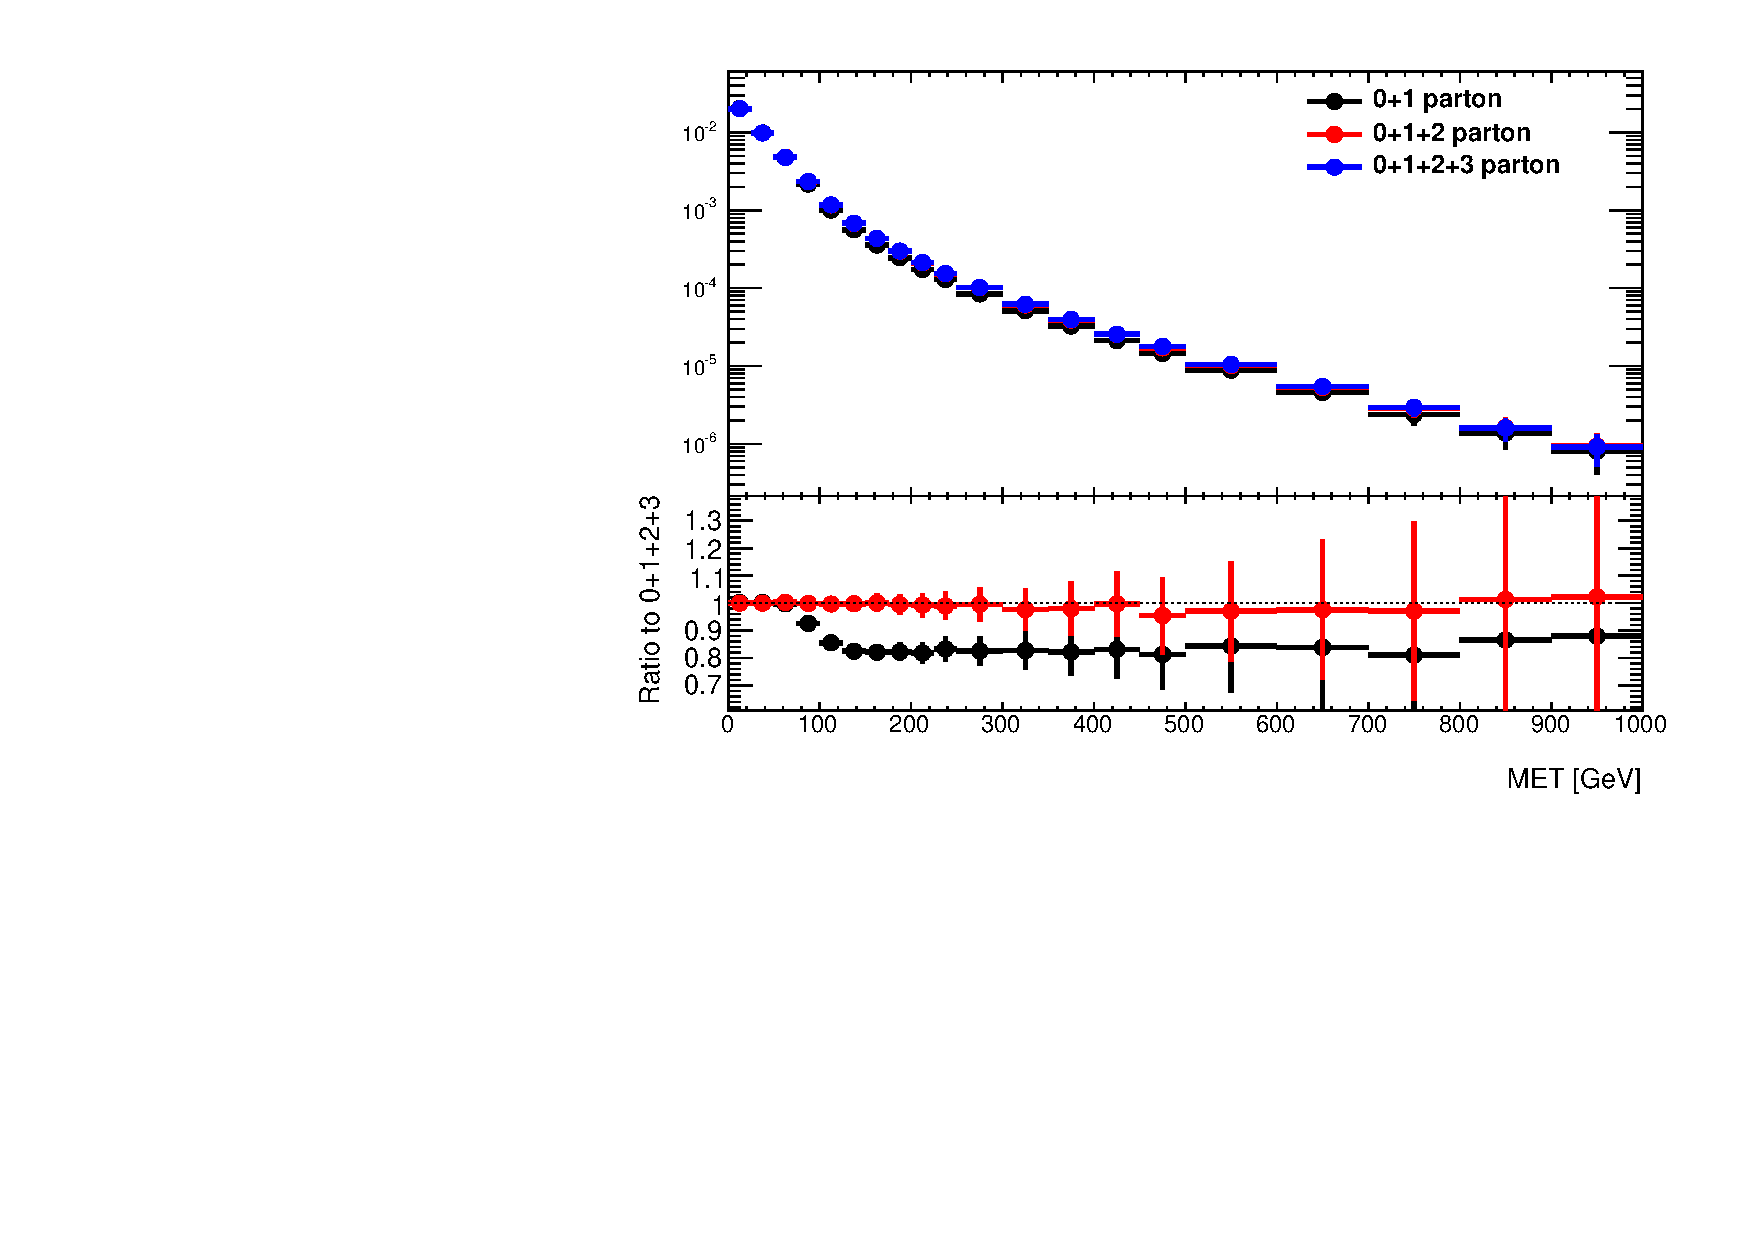
\includegraphics[width=0.48\linewidth]{figures/monojet_appendix/h_MET_3jet.pdf}
	}
	\hfill
%	\subfloat[Transverse momentum of subleading jet]{%
%		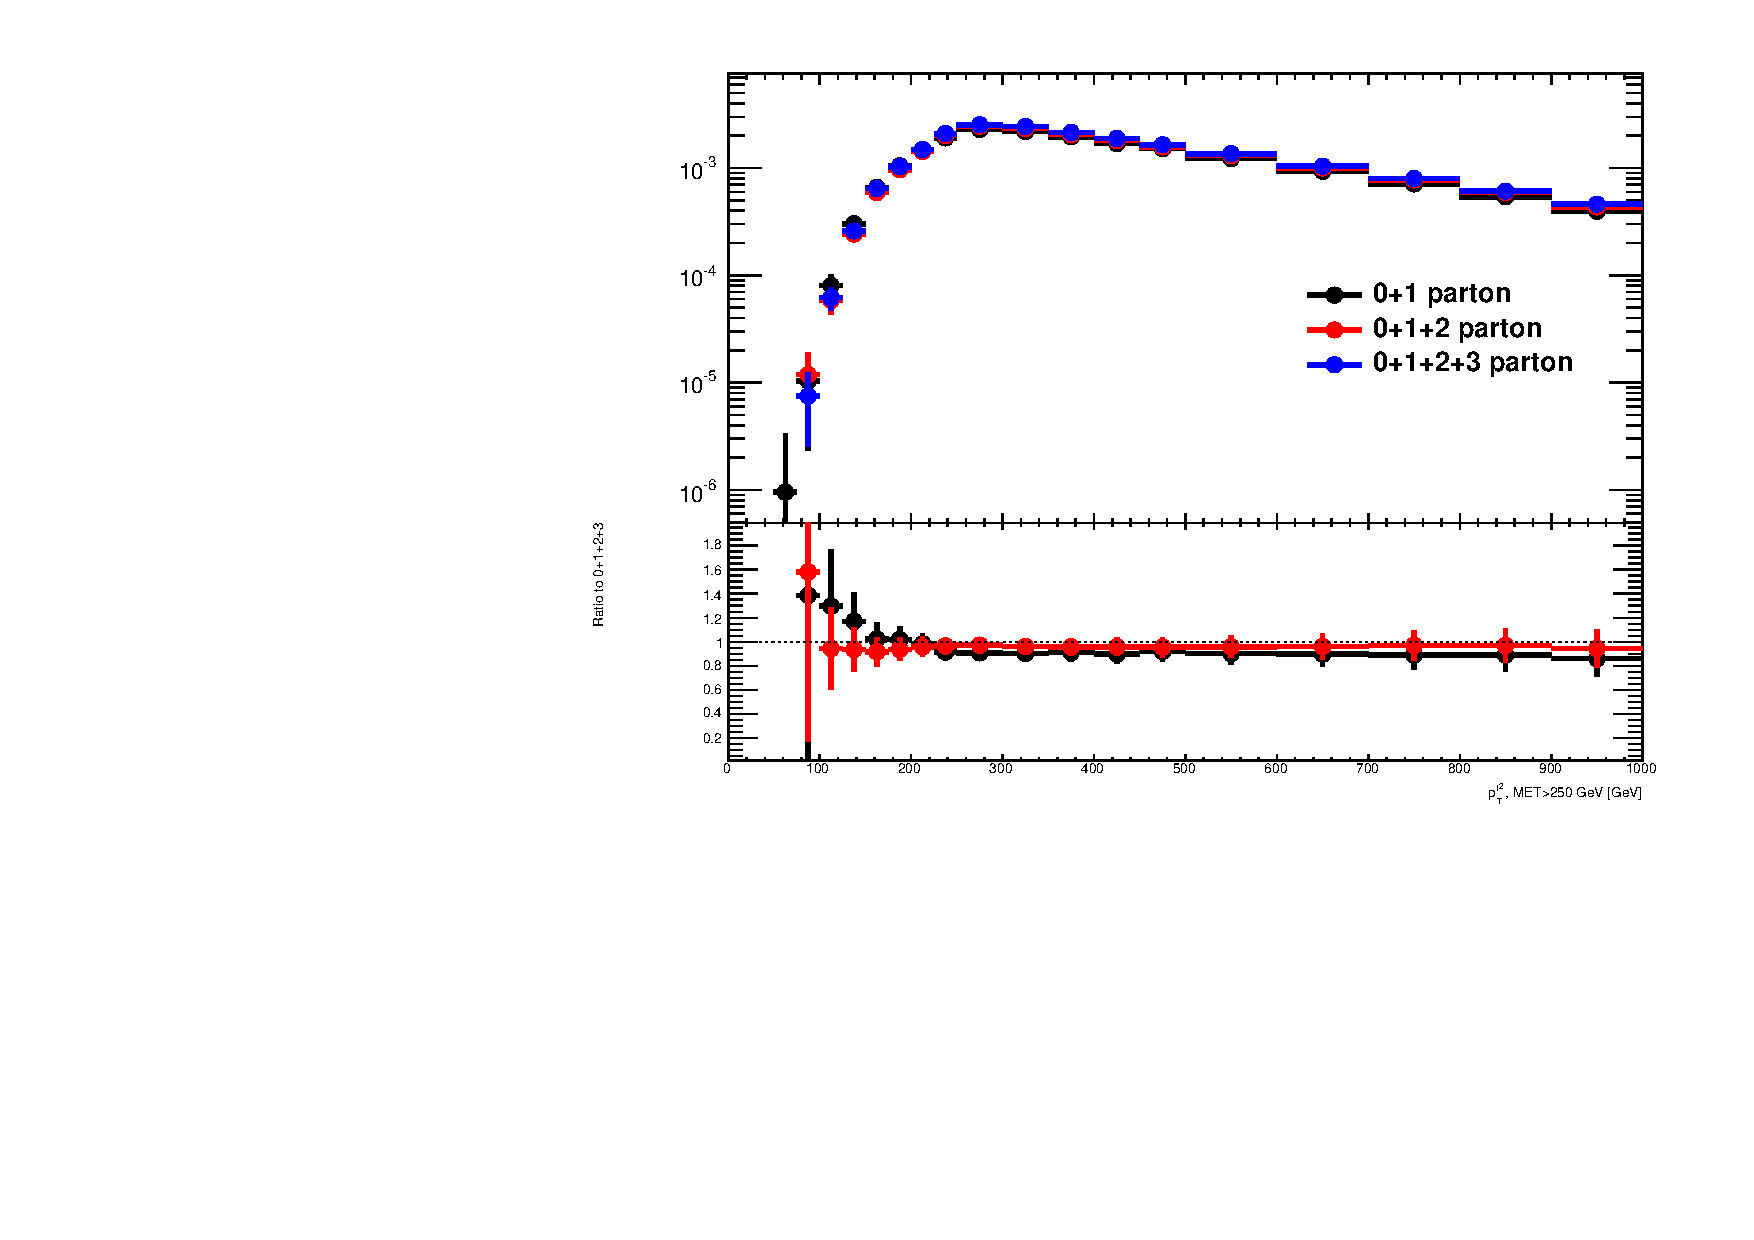
\includegraphics[width=0.48\linewidth]{figures/monojet_appendix/h_pt2_MET250.pdf}
%	}
%	\caption{Kinematics distributions for EFT D5 sample with CKKW matching scale at 80 \gev. 0-, 1-, 2- and 3-parton emission cases are generated separatedly and added together by cross sections.}
	\caption{Missing transverse momentum distributions for EFT D5 sample with CKKW-L matching scale at 80\,\gev produced with maximum 1 (black), 2 (red) and 3 (blue) partons emitted at the generator level. The ratios are shown with respect to the latter sample.}
	\label{fig:RatioKine_D5}
\end{figure}


\begin{figure}[h!]
	\centering  
%	\subfloat[Jet multiplicity, leading jet $p_{T}>30$ \gev]{%
%    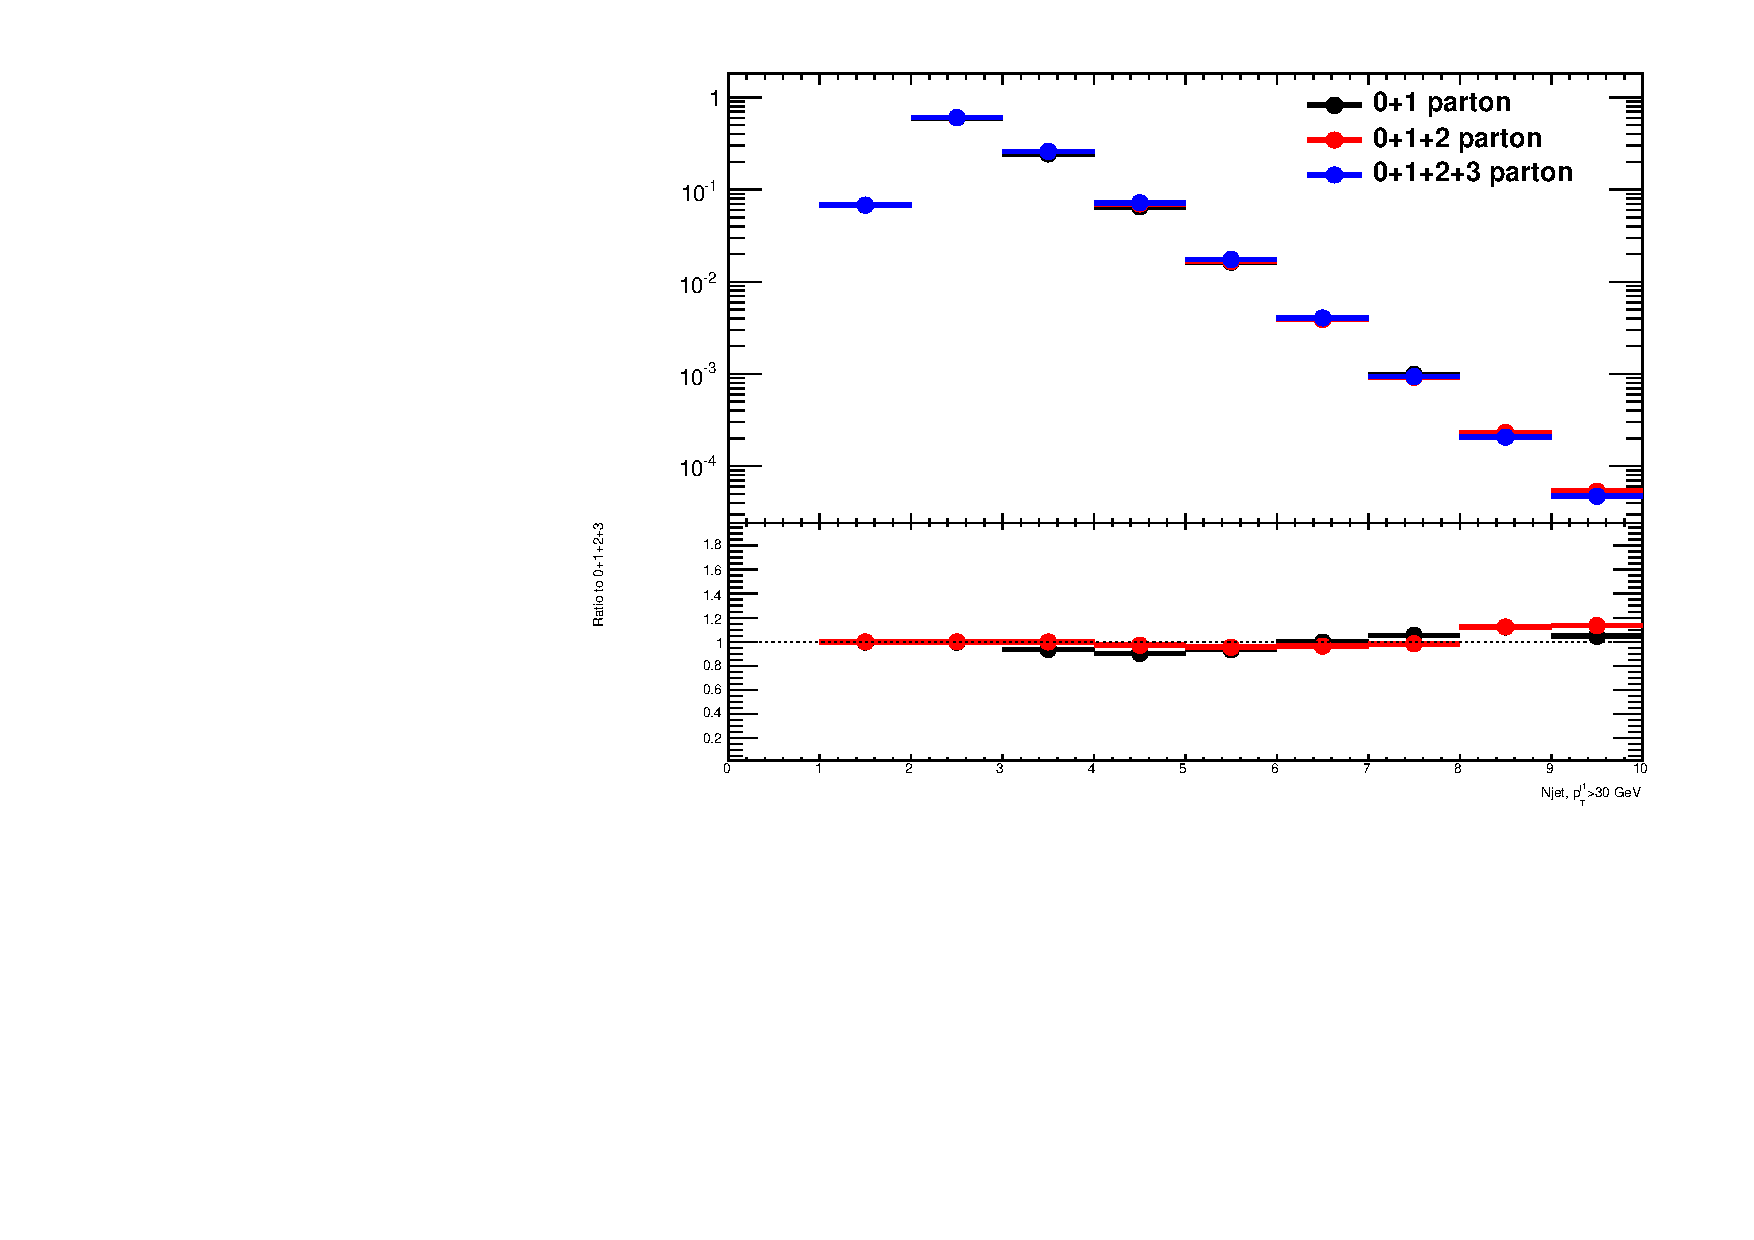
\includegraphics[width=0.48\linewidth]{figures/monojet_appendix/h_njet30.pdf}
%	}
%	\hfill
%	\subfloat[Jet multiplicity, leading jet $p_{T}>80$ \gev]{%
%    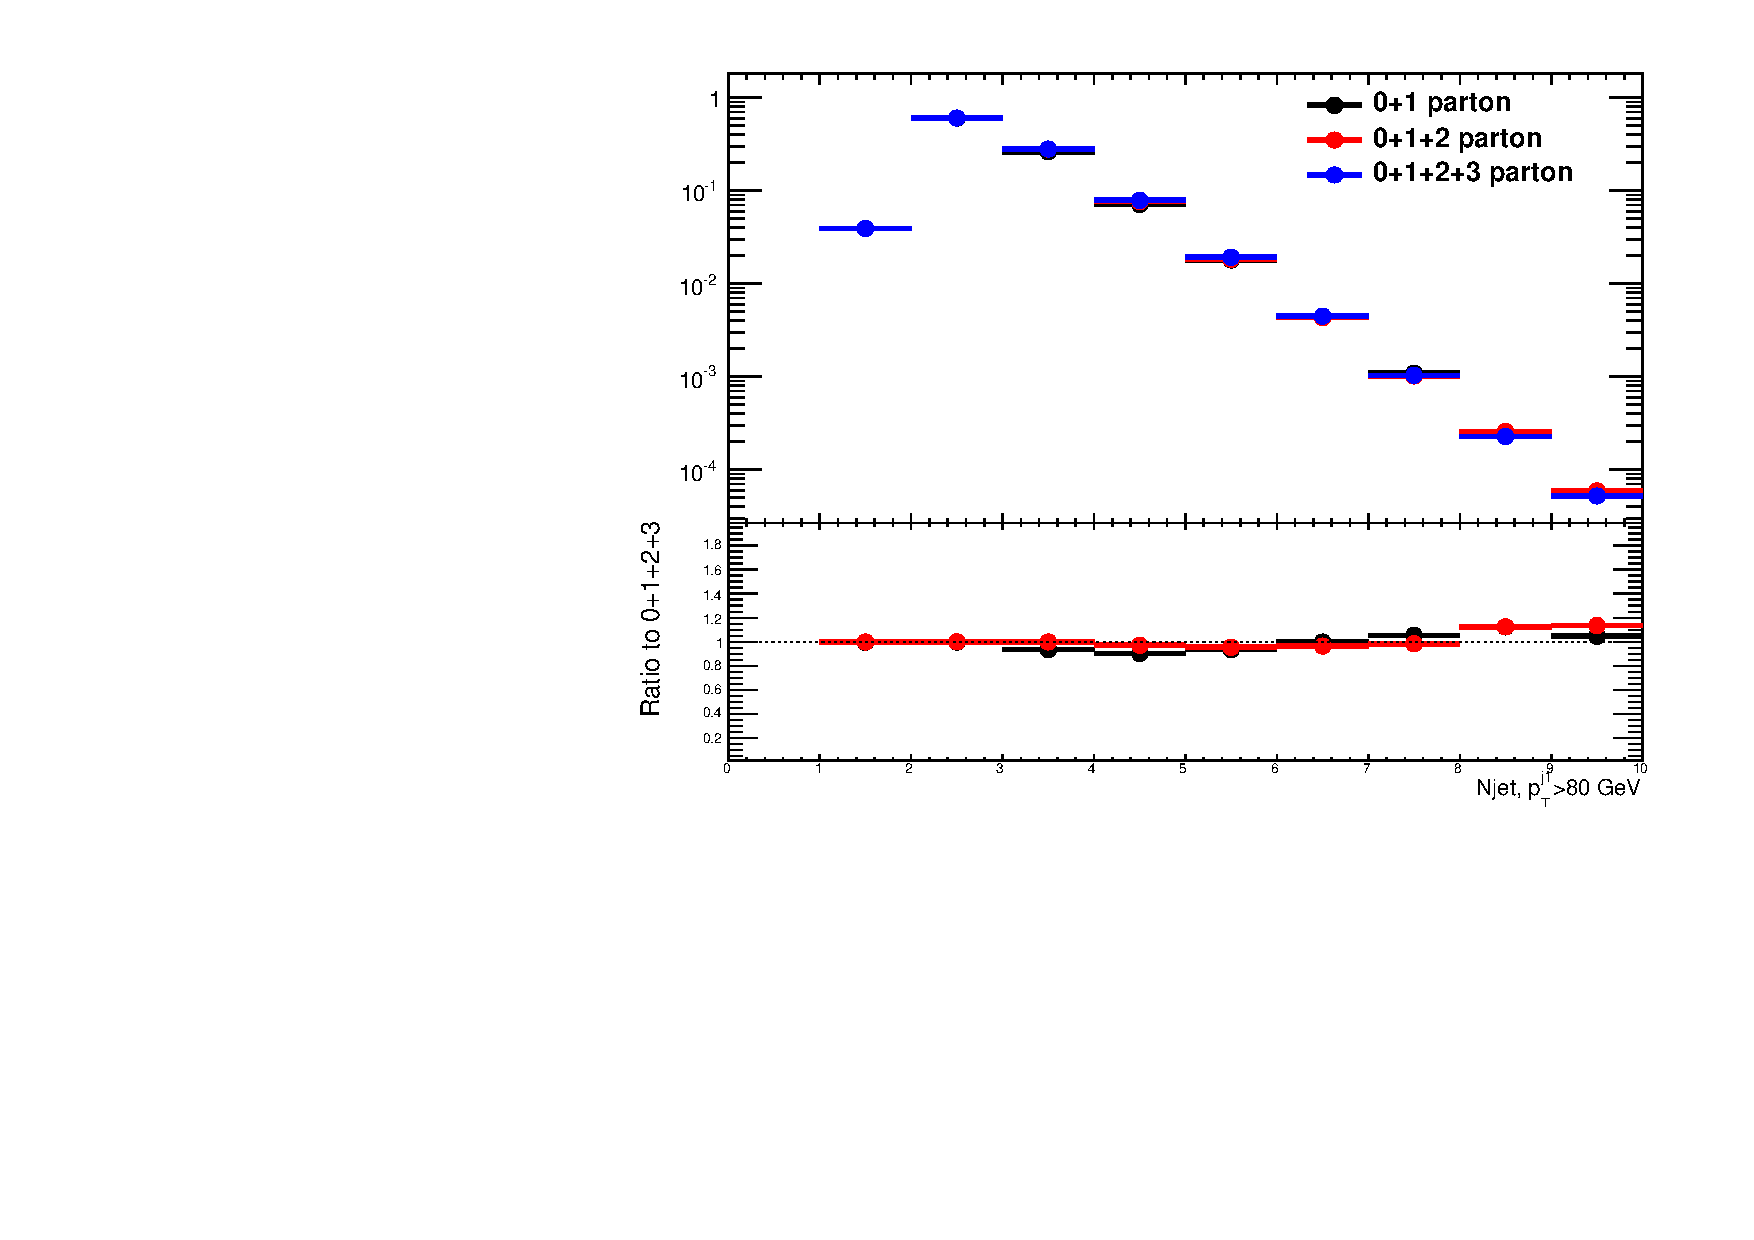
\includegraphics[width=0.48\linewidth]{figures/monojet_appendix/h_njet80.pdf}
%	}
%	\hfill
%	\subfloat[Jet multiplicity, leading jet $p_{T}>250$ \gev]{%
	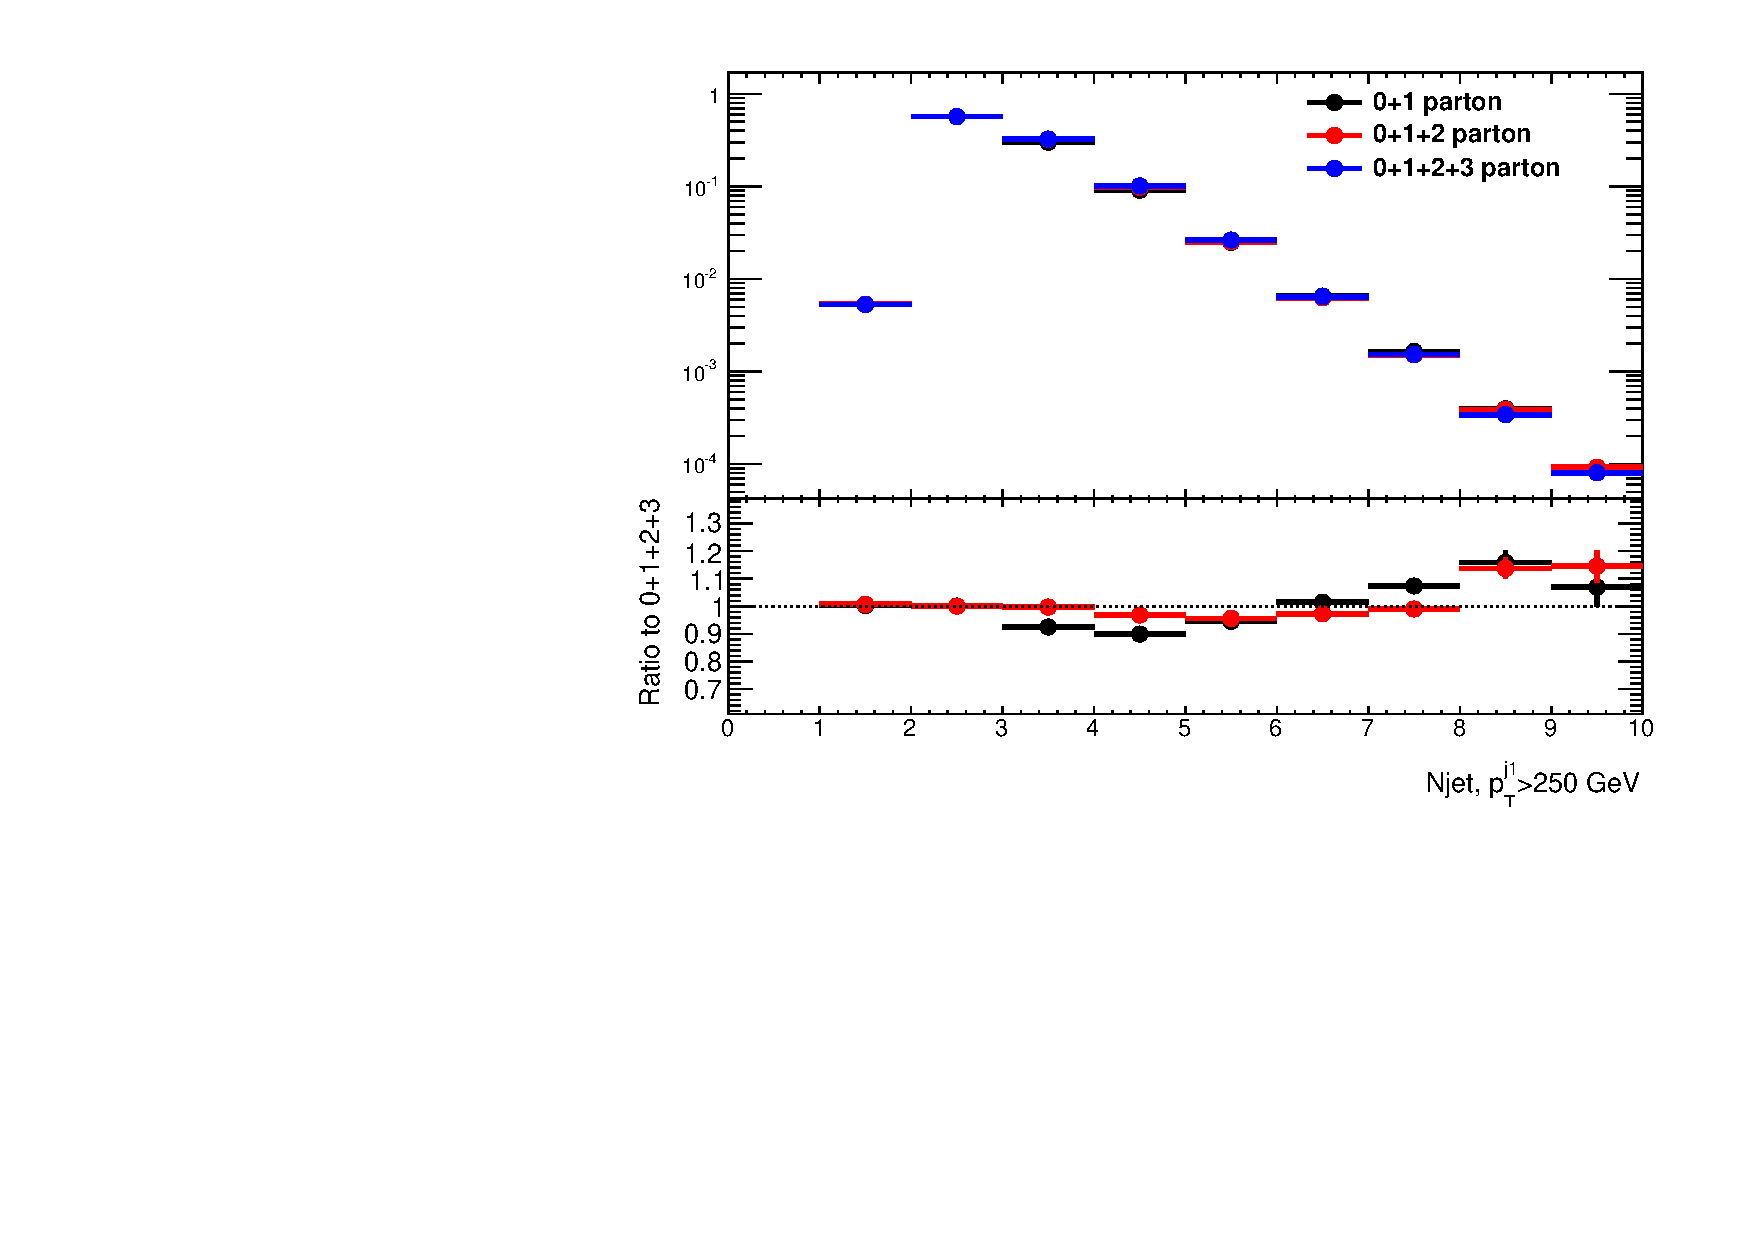
\includegraphics[width=0.8\linewidth]{figures/monojet_appendix/h_njet250.pdf}
%	}
%	\caption{Jet multiplicity distributions for EFT D5 sample with CKKW matching scale at 80 \gev. 0-, 1-, 2- and 3-parton emission cases are generated separatedly and added together by cross sections.}
	\caption{Multiplicity of jets with $\pT>30\,\gev$ and $|\eta<2.8$ for EFT D5 sample with CKKW-L matching scale at 80\,\gev produced with maximum 1 (black), 2 (red) and 3 (blue) partons emitted at the generator level. The ratios are shown with respect to the latter sample. The leading jet $\pT$ is required to be larger than 250\,\gev.}
	\label{fig:RatioKine_D5_2}
\end{figure}


\section{Simplified models for EW final states.}

These models are generated at leading
order with \madgraph 2.2.2, using Pythia8 for the parton shower.
Parameter cards can be found on the Forum SVN repository~\cite{ForumSVN_EW_DMV}.
\Todo{Add models and instructions for other final states}.

\section{Model implementation for mono-Higgs models}

All three Higgs+\MET models are generated at leading
order with \madgraph 2.2.2, using \pythiaEight for the parton shower.
The \madgraph implementations of the scalar and vector models can be found on the Forum SVN 
repository~\cite{ForumSVN_EWMonoHiggs}, while the 2HDM model can be found
at this link~\cite{ForumSVN_EWMonoHiggs_2HDM}.

In all cases, it is recommended not to handle the $h$ decay through \madgraph as
it does not include the proper $h$ branching ratios, or, if using \madgraph, then the 
resulting cross section should be rescaled to match onto the correct branching ratio.

\newthought{\madgraph details for scalar mediator Higgs+MET model}

In this model, the contribution from the $gghS$ box is included through an effective 
Lagrangian evaluated in the large $m_t$ limit. 
This may overestimate the rates of the $h + \MET$ signal~\cite{Haisch:2012kf}, but a full evaluation
is left to future studies. 

\newthought{\madgraph details for 2HDM Higgs+MET model}
  
 The two couplings that can be changed in the implemented model follow the nomenclature below:
 \begin{itemize}
 	\item \texttt{Tb} - $\tan \beta$
 	\item \texttt{gz} - $g_z$, gauge coupling of \Zprime to quarks
 \end{itemize}
 The other couplings are not changed, including \texttt{gx} (the $A \bar \chiDM \chiDM$ coupling) which has little impact on the signal. 
 $\sin \alpha$ is fixed internally such that $\cos (\beta-\alpha) = 0$. 
 The width of the \Zprime and $A$ can be computed automatically within \madgraph. 
 The couplings here don't affect the signal kinematics, so they can be fixed to default values 
 and then the signal rates can be scaled appropriately. 
 
The nomenclature for the masses in the implemented model is:
 \begin{itemize}
 	\item \texttt{MZp} - PDG ID 32 - \Zprime
 	\item \texttt{MA0} - PDG ID 28 - $A$
 	\item \texttt{MX} - PDG ID 1000022 - dark matter particle
 \end{itemize}
 
The other masses are unchanged and do not affect the result. 
 Both $\Zprime \to hZ(\bar \nu \nu)$ and  $\Zprime \to hA(\bar \chiDM \chiDM)$ contribute to the final state, scaling
 different with model parameters. We recommend to generate them separately, 
 and then add the two signal processes together weighted by cross sections.
 % These signals should be generated separately since they have different $\tan \beta, M_A$ dependence.  


\section{Heavy Flavor Models} 
In this particular model we recommend an additional care when choosing
the flavor scheme generation. 
It is found that the best modeling of two $b$-quarks final states is
achieved using a 4-flavor scheme and a massive treatment of the
$b$-quarks \Todo{[TODO: Add reference]}.
% We recommend to use in the generation NNPDF3.0 set (lhaid
%263400).
In addition, we recommend to calculate the cross sections of these
models in the 5-flavor scheme, and as in the $t bar t$ case we provide 
values for the suggested coupling scan in the appendix. 
The PDF used to calculate these cross section is NNPDF3.0 (lhaid 263000). 

\Todo{[TODO: The following figures are placeholders for now and will be added later]}.

\begin{figure}
  \vbox{\hfill}
  \caption{Comparison of the subleading jet $p_T$ and $b$-jet multiplicity
    for $bb$+DM scalar model generated in the 4-flavor (left) and 5-flavor (right)
    schemes, respectively}
\end{figure}

\section{Single Top Models}

Card files for \madgraph are provided on the Forum SVN repository~\cite{ForumSVN_EWMonoTop}, 
corresponding to the Lagrangian from~\cite{AndreaFuksMaltoni}. 
Each coupling constant of this model can be set via the parameter card and 
the blocks which are relevant for the two models used for the experimental searches are described below.
The relevant parameters in the \madgraph parameter cards, also expressed in the notation introduced in the 
previous Section, are as follows for the two models considered.

\begin{enumerate}

\item Resonant scalar model described by the Lagrangian~\eqref{eq:lagrangianResonant}
  \begin{itemize}
  \item \texttt{AQS} and \texttt{BQS}: $3\times 3$ matrices (flavour space) fixing the coupling of the scalar $\phi$ ($S$ stands for scalar) and $down$-type quarks ($Q$ stands for quarks), previously called $a^q/b^q_{SR}$.
  \item \texttt{A12S} and \texttt{B12S}: $3\times 1$ matrices (flavor space) fixing the coupling of the new fermion $\chiDM$ (where $12$ stands for spin-$1/2$ fermion) and $up$-type quarks, previously called $a^{1/2}_{VR}$.
  \end{itemize}  
  
\item Non-resonant vectorial model described by the Lagrangian~\eqref{eq:lagrangianNonResonantVector}
\begin{itemize}
\item \texttt{A1FC} and \texttt{B1FC}: $3\times 3$ matrices (flavor space) fixing the coupling of the vector $V$ ($1$ stands for vector) and $up$-type quarks, previously called $a^1_{FC}$. 
\item particle name: the dark matter candidate $\chiDM$ is not implemented %(as this model assumes $\BR{V}{\chiDM\chiDM}=100\%$)
\end{itemize}

\end{enumerate}

The width of the scalar resonance and of the new vector are set to all allowed decays in the ATLAS implementation,
while the only allowed decay in the CMS implementation to the new fermion and a top quark for the resonant model. 
\Todo{Continue discussion between ATLAS and CMS to reach an agreement, or include instructions to compare results.}

\section{EFT Mono-Higgs implementation}

These models are generated at leading
order with \madgraph 2.2.2, using \pythiaEight for the parton shower. No matching is performed. 
Parameter cards can be found on the Forum SVN repository:~\cite{ForumSVN_EWMonoHiggs} for operators with Higgs+MET final states
and ~\cite{ForumSVN_EWEFTD7} for $W/Z/\gamma$ final states.

\section{Simplified Models of Mono-Higgs}

These models are generated at leading
order with \madgraph 2.2.2, using \pythiaEight for the parton shower. No matching is performed. 
Parameter cards can be found on the Forum SVN 
repository~\cite{ForumSVN_EWMonoHiggs_2HDM, ForumSVN_EWMonoHiggs}.

\subsection{Model implementation for bFDM model}

We simulate the model using the {\tt MG5\_aMC} v2.2.3. The corresponding card files can be found 
on the Forum SVN repository~\cite{ForumSVN_DMSingleB}.

\subsection{Model implementation for VASP models for EW bosons}

These models are generated at leading
order with \madgraph 2.2.2, using Pythia8 for the parton shower.
Parameter cards can be found on the Forum SVN repository~\cite{ForumSVN_EW_DMV}.
\Todo{Add models and instructions for other final states}.
